\section{The information-to-order core and its present boundary}
\label{sec:updated-core-boundary}

Figure~\ref{fig:rqcp-core-mechanism} is the organizing picture for the
foundational part of RQCP-QG.  It contains two logically distinct layers.
Panels 1--5 describe the passage
\begin{equation}
 \text{local quantum observables}
 \longrightarrow
 \text{UCP coarse graining}
 \longrightarrow
 \text{infrared algebra}
 \longrightarrow
 \text{Boolean records},
 \label{eq:updated-information-core}
\end{equation}
while panel 6 asks when response records define a directed acyclic graph.
The abstract statements concern normal process functionals, influence
algebras, Choi--Effros ranges, and center projections.  The dynamical
statements require the explicit models of
Sec.~\ref{sec:closed-loops}.  Conflating those two levels would turn an
existence result into a false universality claim.

A previously used sufficient condition guaranteed acyclicity by prescribing
a Lyapunov function:
\begin{equation}
 i\to j,\quad T(j)>T(i)
 \quad\Longrightarrow\quad
 \text{no directed cycle}.
 \label{eq:updated-lyapunov-sufficient}
\end{equation}
It is no longer the strongest available statement.  In the block-cactus
model, every directed cycle is detected by a bounded local projector, the
defect algebra has an exact contact-process quotient, and extinction of all
defects makes the recorded graph acyclic.  Only after this event is the rank
\begin{equation}
 T_\omega(v)=\max_{p:\,p\to v}|p|
 \label{eq:updated-derived-rank}
\end{equation}
defined.  Thus the model realizes
\[
 \text{local dissipative dynamics}
 \longrightarrow
 \text{cycle extinction}
 \longrightarrow
 \text{DAG}
 \longrightarrow
 \text{derived Lyapunov ranking}.
\]
The distinction is substantive: Eq.~\eqref{eq:updated-derived-rank} is a
property of a realized response record, whereas the semigroup parameter is
the laboratory duration used to generate the record.

The result does not yet compose with the preceding Boolean model.  The
dephasing--exchange graph and the oriented block-cactus graph use different
degrees of freedom and different generators.  A unified model would need an
invariant subalgebra carrying both the Boolean record atoms and the cycle
projectors, plus a proof that the gap controlling record formation is
compatible with the critical closing of the order-formation gap.  That
compatibility is an open theorem, not a matter of relabeling one graph as the
other.

\section{A closed affine order--volume and linearized-gravity bridge}
\label{sec:affine-null-wire-closure}

\textbf{Status: \StatusModel\ for the finite algebraic statements and
\StatusNumerical\ for the archived regulator calculations.}

The affine regulator provides one common-model realization of the
order--volume and gravity interfaces.  The generic order--volume map is
treated separately in Sec.~\ref{sec:updated-order-volume}; the
fully autonomous nonlinear same-update bridge remains open, although
Sec.~\ref{sec:same-update-einstein} closes its finite action-phase
subproblem and Sec.~\ref{sec:three-decisive-chains} closes the relational
clock, quadratic constraint, and balanced-regulator subproblems under their
own visible inputs.  The companion bridge manuscript
\cite{XuOrderVolumeEinstein2026} constructs an affine null-wire regulator in
which order, information volume, metric reconstruction, transverse modular
response, focusing, and tensor completion are interfaces of the same model.
It is not obtained by identifying the block-cactus process of PRL-1 with the
de Sitter detector model of PRL-3.

\subsection{Order and information volume}

Let \(X\subset\mathbb Z^4\) be a finite contractible cubical complex.  Edge
response modes \(a_e\) are acted on by plaquette-local jumps
\begin{equation}
 L_p=\sqrt\kappa\sum_e(d_1)_{pe}a_e ,
 \qquad
 \dot z=-\frac{\kappa}{2}d_1^\dagger d_1z ,
 \label{eq:affine-hodge-flow}
\end{equation}
where \(z_e=\langle a_e\rangle\) and \(d_1d_0=0\).  A fresh-bath
beam-splitter collision realizes each jump; a local product formula gives the
summed semigroup.  Since \(H^1(X)=0\),
\begin{equation}
 z_\infty\in\ker d_1=\operatorname{im}d_0,
 \qquad z_\infty=d_0T .
 \label{eq:affine-exact-form}
\end{equation}
Thresholded responses with a positive limiting margin are therefore oriented
by differences \(T_y-T_x\).  Their directed graph is acyclic because the sum
of strictly positive differences around a cycle would vanish.  The laboratory
semigroup parameter, the recovered rank \(T\), and the affine coordinate
\(x^0\) are distinct.

At vertex \(x\), local dephasing leaves a Boolean record algebra
\(\mathcal A_x^{\rm rec}\simeq\mathbb C^{q_x}\).  Its zero-error classical
capacity gives
\begin{equation}
 \nu(R)=\sum_{x\in R}\log q_x,\qquad
 \mu(R)=\ell_I^4\nu(R).
 \label{eq:affine-information-volume}
\end{equation}
Thus the model produces both an order and a positive additive measure.  The
single dimensionful conversion \(\ell_I^4\) is an explicit calibration.

\subsection{Finite null-frame metric}

The response-active unoriented displacement classes consist of six vectors
of type \((1,\pm1,0,0)\) and permutations, and 24 vectors whose time
component is \(3\) and whose spatial absolute values are
\(\{1,2,2\}\).  For a symmetric tensor \(g\), define
\begin{equation}
 (Ag)_r=v_r^\mu g_{\mu\nu}v_r^\nu .
 \label{eq:affine-design}
\end{equation}
An integer \(9\times9\) minor of \(A\) has determinant \(-32768\).  Hence
\begin{equation}
 \operatorname{rank}A=9,\qquad
 \ker A=\operatorname{span}\{\eta\},\qquad
 \eta=\operatorname{diag}(-1,1,1,1).
 \label{eq:affine-rank-nine}
\end{equation}
The normalized frame has smallest positive singular value \(0.684225689\)
and condition number \(3.635381686\).  The response cone therefore fixes a
conformal Lorentzian metric, while the information volume fixes its scale by
\begin{equation}
 \sqrt{|\det g|}=\mu_0 .
 \label{eq:affine-scale}
\end{equation}
This is a finite cell reconstruction, not a generic curved
metric--measure-limit theorem.  In particular, the affine complex and the
30-class response cone are microscopic inputs.

\subsection{Area response and tensor completion}

Along each of the same 30 directions place a bundle of critical
free-fermion wires.  The fixed-physical-band modular certificate of
Sec.~\ref{sec:loop-modular} is additive over \(N_\perp\) wires.  Since the
transverse cut has \(A_\perp=N_\perp a^2\), division by area cancels
\(N_\perp\) exactly at finite regulator size.  One maximally entangled
\(q_g\)-record pair per cut cell gives
\begin{equation}
 S_\partial=A_\perp\frac{\log q_g}{a^2},
 \qquad
 G_{\rm eff}=\frac{a^2}{4\hbar\log q_g}.
 \label{eq:affine-geff}
\end{equation}
A stated local capacity-exchange channel is primitive and unital within each
conserved capacity sector, so its full sector entropy is stationary to first
order.  The split relation
\(\delta S_\partial+\delta S_{\rm bulk}=0\) additionally uses a full-rank
product reference on the cut and adjacent wire algebras.  Fixed-sector
primitivity does not select this product preparation; its failure is retained
as a measurable stationarity-interface error.

The lattice interval boost and the Dirichlet Green function share the
parabolic weight.  Discrete focusing therefore gives, for every translated
subdiamond and direction \(r\),
\begin{equation}
 \left(
 G_{\mu\nu}^{\rm L}-8\pi G_{\rm eff}T_{\mu\nu}
 \right)v_r^\mu v_r^\nu=\varepsilon_r .
 \label{eq:affine-null-equations}
\end{equation}
The family of translated kernels separates lattice sites.  With
\(E_{\mu\nu}=G_{\mu\nu}^{\rm L}-8\pi G_{\rm eff}T_{\mu\nu}\), the same
rank-nine frame yields
\begin{equation}
 \|P_g^\perp E\|_2
 \le\frac{\|\boldsymbol\varepsilon\|_2}{\sigma_9(A)}
 =1.46151\,\|\boldsymbol\varepsilon\|_2 .
 \label{eq:affine-tensor-error}
\end{equation}
Central finite differences commute, so the linearized lattice Einstein
tensor obeys an exact discrete Bianchi identity.  Conservation of the
number-carrying wire stress leaves only a constant metric mode:
\begin{equation}
 G_{\mu\nu}^{\rm L}
 =8\pi G_{\rm eff}T_{\mu\nu}
 +\Lambda_{\rm int}g_{\mu\nu}.
 \label{eq:affine-einstein}
\end{equation}
A fixed reference boundary may set \(\Lambda_{\rm int}=0\); otherwise it is
retained as an integration constant.

\begin{theorem}[Model-specific order--volume and Einstein closure]
\label{thm:affine-model-closure}
On the contractible affine four-complex, with the stated response cone,
Boolean record cells, decoupled critical-wire bundles, primitive
capacity-exchange channel, stationary product cut--wire reference, linearized
focusing law, and conserved lattice stress,
Eqs.~\eqref{eq:affine-hodge-flow}--\eqref{eq:affine-einstein} form a closed
finite-regulator implication from response dynamics to an acyclic order,
additive information volume, Lorentzian metric, and linearized Einstein tensor
equation.  The nonmetric tensor error is bounded by
Eq.~\eqref{eq:affine-tensor-error}.
\end{theorem}

The theorem closes \(P8_{\rm model}\) and \(P9_{\rm lin,model}\).  It does not
close the general P8 or P9: adjacency and dimension selection, generic curved
convergence, interacting \(3+1\)-dimensional modular universality, nonlinear
focusing, graviton self-interaction, and regulator independence of
\(G_{\rm eff}\) remain open.

\section{A local capacity-reference selection bridge}
\label{sec:capacity-reference-selection}

\textbf{Status: \StatusModel\ for a factorized finite
capacity--complement regulator; \StatusOpen\ for correlated records, the
record--area map, and regulator universality.}

The nonlinear information balance below requires a full-rank boundary
reference whose eigenvalue in an \(n\)-record payload block compensates the
payload multiplicity \(q^n\).  That state need not be installed by an
\(n\)-dependent reset.  The companion reference-selection model
\cite{XuCapacityReference2026} derives it as the unique attractive boundary
state of a sector-blind local random-unitary dynamics.

\subsection{Capacity--complement tokens and local collisions}

Each of \(M\) tokens has a location and a \(q\)-level payload,
\begin{equation}
 \widetilde{\mathcal H}_j
 =\mathbb C^2_{\ell,j}\otimes\mathbb C^q_{p,j},
 \qquad
 \ell\in\{\partial,r\}.
 \label{eq:reference-token}
\end{equation}
Moving a token transfers a fixed information capacity between the visible
boundary and its complement.  Let \(X_d,Z_d\) be generalized Weyl operators.
The product-Weyl twirl and its local generator are
\begin{align}
 \mathcal T_j(\widetilde\rho)
 &=\frac{1}{4q^2}
 \sum_{\substack{a,b=0,1\\c,d=0,\ldots,q-1}}
 W_{abcd}^{(j)}\widetilde\rho W_{abcd}^{(j)\dagger}
 =\frac{I_j}{2q}\otimes\Tr_j\widetilde\rho ,
 \label{eq:reference-twirl}\\
 \widetilde{\mathcal L}^{*}
 &=\gamma\sum_{j=1}^{M}(\mathcal T_j-\mathrm{id}),\qquad
 W_{abcd}=X_2^aZ_2^b\otimes X_q^cZ_q^d .
 \label{eq:reference-generator}
\end{align}
Every collision rate is independent of the total visible-record number.  A
fresh uniformly prepared control cell and the controlled unitary
\(U_j=\sum_\mu|\mu\rangle\langle\mu|\otimes W_\mu^{(j)}\) give a one-pass
unitary dilation, so the twirl is not postulated as a sector reset.

The boundary algebra retains a payload only when its location is
\(\partial\):
\begin{equation}
 \mathcal A_{\partial,j}\simeq\mathbb C\oplus M_q,\qquad
 \mathcal R_j(\widetilde\rho)
 =\Tr_p\langle r|\widetilde\rho|r\rangle
 \oplus\langle\partial|\widetilde\rho|\partial\rangle .
 \label{eq:reference-readout}
\end{equation}
The physical and boundary semigroups intertwine.  On the boundary, the local
expectation replaces token \(j\) by
\(\omega_j=\frac12\oplus I_q/(2q)\), and
\(\mathcal L_\partial^*=\gamma\sum_j(\mathcal E_j^*-\mathrm{id})\).

\begin{theorem}[Capacity-complement reference selection]
\label{thm:capacity-reference-selection}
For every finite \(M\) and \(q\ge2\), the boundary semigroup is primitive and
has the unique stationary state
\begin{equation}
 \omega_\partial
 =\bigotimes_{j=1}^{M}\omega_j
 =2^{-M}\bigoplus_{S\subseteq[M]}q^{-|S|}I_S .
 \label{eq:selected-capacity-reference}
\end{equation}
For every faithful boundary state,
\begin{equation}
 D\!\left(e^{t\mathcal L_\partial^*}\rho\middle\Vert\omega_\partial\right)
 \le e^{-\gamma t}D(\rho\Vert\omega_\partial),
 \label{eq:reference-entropy-contraction}
\end{equation}
with a rate independent of \(M\) and \(q\).  If
\(\widehat N=\sum_j\widehat n_j\) and
\(\widehat A=a_0^2\widehat N\), then
\begin{equation}
 -\log\omega_\partial
 =\frac{\log q}{a_0^2}\widehat A+M\log2 ,
 \qquad
 \operatorname{spec}(-\mathcal L_\partial)
 =\{0,\gamma,\ldots,M\gamma\}.
 \label{eq:selected-modular-area}
\end{equation}
The coefficient \((\log q)/a_0^2\) is unchanged by additive blocking of
microscopic tokens.
\end{theorem}

The stationary state follows by reducing the uniform physical state
\((I_{2q}/2q)^{\otimes M}\).  For a visible set \(S\), tracing the
\(q^{M-|S|}\) complement payload states gives eigenvalue
\(2^{-M}q^{-|S|}\) to every visible payload vector.  Hence the total
\(n\)-record probability is
\(\binom{M}{n}2^{-M}\): payload multiplicity is canceled without appearing
in a collision rate.  Convexity of relative entropy and the quantum Shearer
inequality give Eq.~\eqref{eq:reference-entropy-contraction}; the commuting
local expectations give the spectrum in
Eq.~\eqref{eq:selected-modular-area}
\cite{MullerHermes2016,Capel2021,Dong2026}.

The unbiased location law is falsifiable.  If a visible token has stationary
probability \(p\), the modular increment is
\begin{equation}
 \Delta K(p)=\log\!\left[\frac{q(1-p)}{p}\right],
 \label{eq:reference-bias-control}
\end{equation}
so a pure capacity slope \(\log q\) occurs only at \(p=1/2\).  The finite
model therefore removes a chosen-reference input for the factorized family
\(g_n=\binom{M}{n}\).  It does not derive the location/payload
factorization, unbiased Weyl symmetry, the identification
\(\widehat A=a_0^2\widehat N\), an arbitrary correlated geometric
degeneracy \(g_n\), or a regulator-independent Newton coefficient.

\section{A finite nonlinear information--focusing bridge}
\label{sec:nonlinear-information-focusing}

\textbf{Status: \StatusModel\ for the finite information, optical, and
curved-frame theorems; \StatusConditional\ for nonlinear Einstein closure.}

The affine bridge ends at first order in state exchange and curvature.  The
companion nonlinear bridge \cite{XuNonlinearInformationFocusing2026} asks a
more limited but sharper question: which terms can be retained exactly
before a continuum nonlinear gravitational equation is assumed?  It removes
the entropy-first-law and linearized-focusing truncations in one finite
record regulator and leaves the missing dynamics as a measured Ward defect.
It neither supplies the autonomous order/capacity inputs of the generic
bridge nor identifies a finite-difference equation with general relativity
by definition.

\subsection{Record capacity and the modular area coefficient}

Let the boundary-record Hilbert space be graded by elementary record number,
\begin{equation}
 \mathcal H_{\partial}
 =\bigoplus_{n=0}^{n_{\max}}
 \mathcal G_n\otimes(\mathbb C^{q_g})^{\otimes n},
 \qquad
 \widehat A=a^2\sum_{n=0}^{n_{\max}}nP_n ,
 \label{eq:nonlinear-graded-boundary}
\end{equation}
where \(g_n=\dim\mathcal G_n\), \(P_n\) is the sector projector, and
\(\operatorname{Tr}P_n=g_nq_g^n\).  The capacity-balanced reference is
\begin{equation}
 \rho_{\partial}^0
 =Z_g^{-1}\bigoplus_{n=0}^{n_{\max}}q_g^{-n}I_n,
 \qquad Z_g=\sum_n g_n .
 \label{eq:nonlinear-capacity-reference}
\end{equation}
Its total weight in sector \(n\) is \(g_n/Z_g\): the eigenvalue compensates
the \(q_g^n\) payload multiplicity rather than erasing the geometric
degeneracy \(g_n\).  Blockwise functional calculus gives the exact identity
\begin{equation}
 K_{\partial}^0=-\log\rho_{\partial}^0
 =\frac{\log q_g}{a^2}\widehat A+\log Z_g .
 \label{eq:nonlinear-capacity-modular}
\end{equation}
Consequently,
\begin{equation}
 \frac{1}{4G_{\rm eff}\hbar}=\frac{\log q_g}{a^2},
 \qquad
 G_{\rm eff}=\frac{a^2}{4\hbar\log q_g}.
 \label{eq:nonlinear-geff}
\end{equation}
Unlike a fit of an area law, Eq.~\eqref{eq:nonlinear-geff} is fixed once the
reference \eqref{eq:nonlinear-capacity-reference} is selected.
Theorem~\ref{thm:capacity-reference-selection} supplies exactly such a unique
attractive state for the factorized family
\(g_n=\binom{M}{n}\), with a size-independent contraction rate.  The
nonlinear theorem here allows arbitrary \(g_n\), however, and it does not
couple the selection semigroup to the record--bulk--geometry update.
Selection for correlated record geometry, the record--area identification,
and regulator universality therefore remain open.

\subsection{Exact finite information balance}

Let \(\rho_b^0\) be any full-rank bulk reference and
\(\rho_0=\rho_{\partial}^0\otimes\rho_b^0\).  For an arbitrary unitary
record--bulk exchange \(U\), write
\(\rho=U\rho_0U^\dagger\) and
\(K_b^0=-\log\rho_b^0\).  Entropy invariance and the product-reference
chain rule give
\begin{align}
 \frac{\Delta A}{4G_{\rm eff}\hbar}
 +\Delta\langle K_b^0\rangle
 &=D(\rho\Vert\rho_0)\nonumber\\
 &=D(\rho_{\partial}\Vert\rho_{\partial}^0)
 +D(\rho_b\Vert\rho_b^0)
 +I_\rho(\partial{:}b)\nonumber\\
 &:=\mathcal R_{\rm info}.
 \label{eq:nonlinear-finite-information}
\end{align}
No exchange-angle expansion enters.  All three terms in
\(\mathcal R_{\rm info}\) are nonnegative.  For
\(U_\theta=e^{-i\theta V}\), the first derivative at \(\theta=0\) vanishes
and the Hessian is the Bogoliubov--Kubo--Mori information metric:
\begin{equation}
 \mathcal R_{\rm info}(\theta)
 =\frac{\theta^2}{2}
 g_{\rm BKM,\rho_0}
 \!\left(-i[V,\rho_0],-i[V,\rho_0]\right)+O(\theta^3).
 \label{eq:nonlinear-bkm}
\end{equation}
The entropy first law is therefore recovered as the tangent statement of an
exact finite balance; the information metric is the first omitted term, not
an optional correction \cite{Petz1996,Lashkari2016}.

\subsection{Exact discrete nonlinear optics}

For affine steps \(\lambda_j=ja\), let \(J_j\) be the transverse Jacobi map
and define the finite regulator by
\begin{equation}
 J_{j+1}-2J_j+J_{j-1}=-a^2\mathcal R_jJ_j ,
 \label{eq:nonlinear-jacobi}
\end{equation}
where \(\mathcal R_j\) is the symmetric optical tidal matrix.  Before the
first caustic, define
\begin{equation}
 F_j=J_jJ_{j-1}^{-1}=\mathbf1+aB_j .
\end{equation}
Equation~\eqref{eq:nonlinear-jacobi} is then exactly equivalent to
\begin{align}
 B_{j+1}
 &=B_j(\mathbf1+aB_j)^{-1}-a\mathcal R_j,
 \label{eq:nonlinear-riccati}\\
 \frac{B_{j+1}-B_j}{a}
 &=-B_j^2(\mathbf1+aB_j)^{-1}-\mathcal R_j ,
 \label{eq:nonlinear-discrete-raychaudhuri}\\
 \frac{A_j}{A_{j-1}}
 &=\det(\mathbf1+aB_j).
 \label{eq:nonlinear-area-update}
\end{align}
The quadratic expansion, shear, and twist terms arise from the Riccati
transform; they are not appended to a scalar area law.  The continuum
expansion of Eq.~\eqref{eq:nonlinear-discrete-raychaudhuri} gives the full
Raychaudhuri equation.  At a caustic the Riccati chart fails while the doubled
transfer relation for \((J_{j+1},J_j)\) remains regular.  A global extension
requires a Lagrangian-Grassmannian or Maslov-index description and is kept
open.

\subsection{Curved null frames and tensor stability}

The same 30 rational null directions used in the affine construction may be
transported by an arbitrary invertible coframe.  Let
\begin{equation}
 g=e^T\eta e,\qquad k_r=e^{-1}v_r .
 \label{eq:nonlinear-curved-frame}
\end{equation}
For a symmetric tensor \(S\), let \(A_gS\) be the vector of row-normalized
quadratic forms \(S_{\mu\nu}k_r^\mu k_r^\nu\), with the symmetric-tensor
vectorization chosen isometrically in the Frobenius norm.  Congruence by
\(e^{-1}\) is invertible, so the affine rank certificate implies
\begin{equation}
 \operatorname{rank}A_g=9,\qquad
 \ker A_g=\operatorname{span}\{g\}.
 \label{eq:nonlinear-curved-rank}
\end{equation}
If \(\sigma_9(A_g)\) is the smallest nonzero singular value and
\(A_gS=\epsilon\), then
\begin{equation}
 \inf_{\phi\in\mathbb R}\|S-\phi g\|_F
 \le\frac{\|\epsilon\|_2}{\sigma_9(A_g)} .
 \label{eq:nonlinear-curved-stability}
\end{equation}
Thus the finite frame remains informationally complete for the trace-free
tensor after arbitrary local coframe deformation.  Curvature changes its
conditioning, not its rank.  Spacetime dimension and the reference
direction set are still regulator inputs.

\subsection{The finite Ward-defect equation}

For a small null diamond in direction \(r\), use a fixed Green weight to
define the integrated contractions \(Q_R^{(r)}\) and \(Q_T^{(r)}\).  The
exact Jacobi area and the bulk modular response define separately measurable
remainders:
\begin{align}
 \Delta A^{(r)}
 &=-A_{\perp,r}Q_R^{(r)}+\varepsilon_{\rm foc}^{(r)},\label{eq:nonlinear-foc-def}\\
 \Delta\langle K_b^0\rangle^{(r)}
 &=\frac{2\pi}{\hbar}A_{\perp,r}Q_T^{(r)}
 +\varepsilon_{\rm mod}^{(r)}.\label{eq:nonlinear-mod-def}
\end{align}
Substitution into Eq.~\eqref{eq:nonlinear-finite-information} yields the exact
finite identity
\begin{equation}
 \boxed{\begin{aligned}
 Q_R^{(r)}-8\pi G_{\rm eff}Q_T^{(r)}
 ={}&\frac{\varepsilon_{\rm foc}^{(r)}}{A_{\perp,r}}\\
 &+\frac{4G_{\rm eff}\hbar}{A_{\perp,r}}
 \left(\varepsilon_{\rm mod}^{(r)}
 -\mathcal R_{\rm info}^{(r)}\right).
 \end{aligned}}
 \label{eq:nonlinear-null-defect}
\end{equation}
Variation of the coframe and Green weight across a shrinking diamond adds a
separately defined localization defect
\(\varepsilon_{\rm loc}^{(r)}\) to the projection data in
Eq.~\eqref{eq:nonlinear-curved-stability}.  The zero-defect target at finite
resolution is therefore the Ward relation
\begin{equation}
 \mathcal R_{\rm info}^{(r)}
 =\varepsilon_{\rm mod}^{(r)}
 +\frac{\varepsilon_{\rm foc}^{(r)}}
 {4G_{\rm eff}\hbar},
 \label{eq:nonlinear-ward-target}
\end{equation}
together with a controlled localization limit.  Equation
\eqref{eq:nonlinear-ward-target} is not imposed in the companion model.  It
is the microscopic identity required of a common
record--matter--geometry update.

\begin{theorem}[Finite nonlinear remainder bridge]
\label{thm:finite-nonlinear-remainder}
For the capacity-balanced reference
\eqref{eq:nonlinear-capacity-reference}, a full-rank product bulk reference,
an arbitrary unitary record--bulk exchange, the discrete Jacobi regulator
\eqref{eq:nonlinear-jacobi} before its first caustic, and the coframe-
transported 30-direction null design, Eqs.
\eqref{eq:nonlinear-capacity-modular},
\eqref{eq:nonlinear-finite-information},
\eqref{eq:nonlinear-riccati}--\eqref{eq:nonlinear-area-update},
\eqref{eq:nonlinear-curved-rank}--\eqref{eq:nonlinear-curved-stability}, and
\eqref{eq:nonlinear-null-defect} hold exactly at finite regulator size.
\end{theorem}

The theorem closes \(P9_{\rm nonlinear\ remainder,model}\), not P9.  If the
normalized right-hand side of Eq.~\eqref{eq:nonlinear-null-defect} and the
localization defect vanish for all frame directions, then the curvature--
stress difference is a cell-dependent multiple \(\phi_xg_{\mu\nu}(x)\).
Turning that local scalar freedom into one constant is a separate finite
completion problem.  It can be controlled quantitatively, but only after the
response tensor is identified with the geometric Euler derivative of the
same process.

\section{A quantitative finite Ward--Bianchi completion bridge}
\label{sec:ward-bianchi-completion}

\textbf{Status: \StatusAbstract\ for the finite completion theorem and
\StatusNumerical\ for the periodic four-lattice certificate;
\StatusOpen\ for the constitutive Ward identification and its uniform
interacting continuum limit.}

Let \(\mathcal S_h\) and \(\mathcal V_h\) be finite Hilbert spaces of
symmetric tensor and covector fields.  A metric field \(g_x\) defines
\[
 M_g\phi=\{\phi_xg_x\}_{x\in C_h}.
\]
Let \(A_h:\mathcal S_h\to\mathcal Y_h\) collect normalized contractions with
a local null frame and assume the exact finite completeness condition
\begin{equation}
 \ker A_h=\operatorname{ran}M_g,\qquad
 A_h^+A_h=P_g^\perp .
 \label{eq:finite-null-kernel}
\end{equation}
Thus null data determine every nonmetric component but are blind to an
independent scalar \(\phi_x\) at each cell.  Let
\(B_h:\mathcal S_h\to\mathcal V_h\) be the covariant divergence constructed
from the same finite geometry, with
\begin{equation}
 B_hM_g=D_h,\qquad
 \|\phi-\bar\phi\|
 \le\lambda_h^{-1/2}\|D_h\phi\|,
 \quad \lambda_h>0 .
 \label{eq:finite-compatible-poincare}
\end{equation}
The second relation is a scalar Poincar\'e estimate after removal of the
constant mode.

For noisy direction-resolved data
\[
 y=A_hW+n,\qquad \|n\|\le\nu,\qquad
 \widehat E=A_h^+y,
\]
define the two reconstructed budgets
\begin{equation}
 \eta_0=\|\widehat E\|+\|A_h^+\|\nu,\qquad
 \eta_1=\|B_h\widehat E\|+\|B_hA_h^+\|\nu .
 \label{eq:finite-reconstructed-budgets}
\end{equation}

\begin{theorem}[Noisy finite Ward--Bianchi completion]
\label{thm:ward-bianchi-completion}
Assume Eqs.~\eqref{eq:finite-null-kernel} and
\eqref{eq:finite-compatible-poincare}.  If
\(\|B_hW\|\le\varepsilon_{\rm W}\), then there is one constant
\(\bar\phi\) such that
\begin{equation}
 \boxed{
 \|W-M_g\bar\phi\|
 \le
 \eta_0+\frac{\|M_g\|}{\sqrt{\lambda_h}}
 \left(\varepsilon_{\rm W}+\eta_1\right).}
 \label{eq:ward-bianchi-completion}
\end{equation}
\end{theorem}

\begin{proof}
Write \(W=M_g\phi+E\), with
\(E=P_g^\perp W=A_h^+A_hW\).  The noisy reconstruction gives
\(\|E\|\le\eta_0\) and \(\|B_hE\|\le\eta_1\).  Compatibility then yields
\[
 \|D_h\phi\|
 =\|B_hM_g\phi\|
 \le\|B_hW\|+\|B_hE\|
 \le\varepsilon_{\rm W}+\eta_1.
\]
Apply the Poincar\'e estimate and
\(\|M_g(\phi-\bar\phi)\|\le\|M_g\|\|\phi-\bar\phi\|\).
\end{proof}

The Ward residual can itself be tied to one finite process functional.
Let \(\Gamma_h(z,m)\) depend differentiably on geometric and matter
variables.  For the tangent generators \(R_z\xi,R_m\xi\), define Euler
covectors \(\mathcal E_z=D_z\Gamma_h\),
\(\mathcal E_m=D_m\Gamma_h\) and the finite symmetry defect
\(\delta_{\rm sym}\) by differentiation along the joint transformation.
The chain rule gives the exact identity
\begin{equation}
 R_z^*\mathcal E_z+R_m^*\mathcal E_m
 =\delta_{\rm sym}.
 \label{eq:finite-noether-defect}
\end{equation}
Consequently, if
\begin{equation}
 W=\mathcal E_z,\qquad B_h=R_z^*,
 \label{eq:constitutive-ward-identification}
\end{equation}
then
\begin{equation}
 \varepsilon_{\rm W}
 \le\|\delta_{\rm sym}\|
 +\|R_m^*\|\,\|\mathcal E_m\|.
 \label{eq:finite-ward-budget}
\end{equation}
More generally, retain the constitutive defect
\[
 C_h=W-\mathcal E_z,\qquad
 \|C_h\|\le\varepsilon_{\rm cons}^{(0)},\qquad
 \|B_hC_h\|\le\varepsilon_{\rm cons}^{(1)} .
\]
The same proof gives the explicit certificate
\begin{align}
\inf_{\bar\phi\in\mathbb R}
\|\mathcal E_z-M_g\bar\phi\|
\le{}&\eta_0+\varepsilon_{\rm cons}^{(0)}
+\frac{\|M_g\|}{\sqrt{\lambda_h}}\bigl[
\eta_1+\varepsilon_{\rm cons}^{(1)}
\nonumber\\[-2pt]
&+\|\delta_{\rm sym}\|
+\|R_m^*\|\,\|\mathcal E_m\|\bigr].
\label{eq:finite-constitutive-certificate}
\end{align}
Equations~\eqref{eq:ward-bianchi-completion} and
\eqref{eq:finite-constitutive-certificate} put null tomography, constitutive
mismatch, finite symmetry breaking, off-shell matter, measurement noise, and
scalar conditioning in one error budget \cite{XuWardBianchi2026}.

The irreducible open arrow is the simultaneous decay of the two
constitutive defects in Eq.~\eqref{eq:finite-constitutive-certificate};
Eq.~\eqref{eq:constitutive-ward-identification} is their exact endpoint.
Gauge covariance cannot prove that the tensor assembled from the information
and optical sides of Eq.~\eqref{eq:nonlinear-null-defect} approaches the Euler
covector of the same functional, either before or after applying the spatial
divergence.  That is the microscopic information--geometry constitutive Ward
relation.  Nor may a holonomy identity be substituted for it.  Products of
face holonomies obey exact nonlinear lattice Bianchi identities
\cite{Batrouni1982,HamberKagel2004}, and finite Noether laws have exact
discrete formulations \cite{Skopenkov2023,Arrighi2023}; nevertheless, a
generic curved Regge lattice on a fixed triangulation does not have exact
vertex-displacement symmetry \cite{BahrDittrich2009}.  Kinematic holonomy
closure and dynamical diffeomorphism symmetry are different statements.

The companion certificate uses a periodic physical-side-one \(L^4\)
lattice, backward-incidence divergence, and the 30 rational null directions
of the earlier bridges.  Its row-normalized design has rank nine,
\(\ker A_h=\mathbb R\eta\), and
\(\sigma_9=0.8498365856\).  All 96 independently generated noisy smooth
fields on \(L=4,6,8,10\) satisfy
Eq.~\eqref{eq:ward-bianchi-completion}; the certified-bound to
actual-error ratios range from \(1.586\) to \(6.776\).  A frozen refinement
family over
\(L=4,6,8,10,12,16\) has actual and certified powers \(2.000\) and \(2.057\).
Two exact controls expose nonredundancy:
\[
 W(x)=\phi(x)\eta
 \quad\Longrightarrow\quad
 A_hW=0\ \text{but}\ B_hW\ne0,
\]
whereas a constant trace-free anisotropy has
\(B_hW=0\) but \(A_hW\ne0\).  Only a constant metric mode makes both
residuals vanish.

For a refinement family, the finite theorem gives a continuum-use
corollary.  If \(\|M_g\|\) and \(\|A_h^+\|\) remain bounded,
\(\lambda_h\) stays bounded below in the physical normalization, and
\[
\|A_h^+\|\nu_h+\|B_hA_h^+\|\nu_h
+\|\widehat E_h\|+\|B_h\widehat E_h\|
+\|\delta_{{\rm sym},h}\|
+\|R_{m,h}^*\|\,\|\mathcal E_{m,h}\|
\longrightarrow0 ,
\]
then, under the exact constitutive identification,
\[
 \inf_{\bar\phi\in\mathbb R}\|W_h-M_{g,h}\bar\phi\|\longrightarrow0.
\]
For an approximate identification, the two constitutive terms in
Eq.~\eqref{eq:finite-constitutive-certificate} must vanish as well.
This does not prove those uniform hypotheses.  It identifies exactly which
conditioning or dynamical defect would obstruct the limit and leaves the
constant metric mode to boundary or cosmological dynamics.

\section{A same-update finite Einstein--matter closure}
\label{sec:same-update-einstein}

\textbf{Status: \StatusModel\ for the local Ramsey action-phase identity and
its central-difference theorem; \StatusNumerical\ for the nonlinear FLRW and
four-dimensional tensor refinements; \StatusOpen\ for dynamical selection of
the action and a regulator-independent interacting limit.}

The constitutive quantities in
Eq.~\eqref{eq:finite-constitutive-certificate} need not remain independently
specified.  Let one finite regulator have variables \(q=(z,m)\), positive
cell weights \(\omega_{a,\alpha}\), and one declared local phase functional
\begin{equation}
 \Gamma_a(q)=\sum_{\alpha\in\Lambda_a}
 \omega_{a,\alpha}\gamma_{a,\alpha}(q_{\mathcal N(\alpha)}),
 \qquad
 \widehat\Gamma_a=\sum_q\Gamma_a(q)|q\rangle\langle q|.
 \label{eq:same-update-local-action}
\end{equation}
A fresh ancilla coherently controls the two interventions
\(q\mapsto q\pm\varepsilon e_\alpha\), applies
\(U_a(s)=e^{-is\widehat\Gamma_a}\), and undoes the intervention.  Its
\(X/Y\) coherence gives the operational score
\begin{equation}
 W^\varepsilon_{a,\alpha}
 =\frac{\Gamma_a(q+\varepsilon e_\alpha)
              -\Gamma_a(q-\varepsilon e_\alpha)}
        {2\varepsilon\omega_{a,\alpha}} ,
 \label{eq:same-update-operational-score}
\end{equation}
without evaluating the analytic derivative
\(\mathcal E_a=D\Gamma_a\).

\begin{theorem}[Same-update response--Euler certificate]
\label{thm:same-update-einstein}
Suppose the normalized third-derivative densities of \(\Gamma_a\) and the
first finite differences of their central-difference remainder field are
bounded by \(M_{0,a}\) and \(M_{1,a}\).  Then
\begin{equation}
 \|W_a^\varepsilon-\mathcal E_a\|_a
 \le\frac{\varepsilon^2}{6}M_{0,a},
 \qquad
 \|B_a(W_a^\varepsilon-\mathcal E_a)\|_a
 \le\varepsilon^2M_{1,a}.
 \label{eq:same-update-two-defects}
\end{equation}
For a quadratic phase action both defects vanish exactly.  Let \(r_a\)
denote the right-hand side of
Eq.~\eqref{eq:finite-constitutive-certificate} after substituting these two
budgets.  If one additional operational volume covector \(v_a\) satisfies
\(v_a(M_g1)=1\), \(\|v_a\|\le c_{v,a}\), and
\(|v_a(W_a^\varepsilon)|\le\eta_{V,a}\), then the complete geometric Euler
covector obeys
\begin{equation}
 \boxed{\;
 \|\mathcal E_{z,a}\|_a
 \le (1+c_{v,a})r_a+\eta_{V,a}
       +c_{v,a}\frac{\varepsilon^2M_{0,a}}{6}\; .}
 \label{eq:same-update-full-certificate}
\end{equation}
\end{theorem}

The first two inequalities are Taylor's formula with its integral remainder,
retained as a lattice field before applying \(B_a\).  For the last inequality,
the null--Ward argument gives
\(\mathcal E_{z,a}=M_g\bar\phi_a+\rho_a\) with
\(\|\rho_a\|_a\le r_a\).  Applying \(v_a\) controls
\(|\bar\phi_a|\), including its response and central-difference errors, and
then the triangle inequality proves
Eq.~\eqref{eq:same-update-full-certificate}.  Without \(v_a\), null and
divergence data still leave the constant metric mode undetermined.

The companion calculation \cite{XuSameUpdateEinstein2026} keeps the
operational and analytic pipelines independent.  In a midpoint discretization
of the Einstein--massless-scalar FLRW action, the response--Euler field and
derivative defects converge with fitted powers \(2.994\) and \(2.915\);
the finite symmetry and full Einstein--scalar residuals converge with powers
\(2.104\) and \(1.962\).  On a periodic \(L^4\) transverse-traceless
lattice the quadratic Ramsey--Euler defect is below
\(2.8\times10^{-14}\), the null and null-plus-volume frames have ranks nine
and ten with
\(\sigma_9=\sigma_{10}=0.8498365856\), and the complete tensor residual has
power \(1.888\).  A quartic FLRW phase term and a quadratic TT term inserted
only in the Ramsey branch leave respective defects above
\(3.37\times10^{-2}\) and \(1.27\times10^{-3}\).  These controls exclude
agreement obtained by projecting the response into an Einstein sector after
measurement.

The result removes the finite-model sub-assumption \(A11S\), not the general
gravitational assumption \(A11\).  Equation
\eqref{eq:same-update-local-action} already contains an Einstein--matter phase
action on a four-dimensional Lorentzian regulator.  The Ramsey theorem
certifies the Euler equation of that action; it does not explain why a less
structured autonomous quantum process selects the action, its variables, or
its normalization.  A general continuum claim additionally requires uniform
control of \(M_{0,a},M_{1,a},A_a^+,\lambda_a^{-1/2}\), phase-unwrapping
resources, finite symmetry and matter residuals, and the regulator response
coefficient.

The remaining steps are:
\begin{enumerate}[label=(N\arabic*)]
\item couple the selected factorized reference to the same
record--matter--geometry update, extend its contraction theorem to correlated
record geometry, and derive the record--area map;
\item prove an interacting fixed-physical-band modular theorem for local
wave packets;
\item replace the prescribed phase action in
Theorem~\ref{thm:same-update-einstein} by one autonomous
record--matter--Lorentz-holonomy dynamics whose infrared phase is proved to
approach the Einstein--Hilbert form, while retaining independent response and
variation pipelines;
\item bound the same update's finite symmetry defect and matter
equation-of-motion residual, while keeping the exact cell-holonomy Bianchi
identity as a distinct geometric consistency check;
\item continue the optical and record data through caustics with a
patch-independent Maslov index; and
\item prove a uniform shrinking-diamond and regulator-independence limit.
\end{enumerate}
These are stronger requirements than discretizing Einstein's equation.  They
ask the quantum information cost, optical nonlinearity, and conservation
identities to be consequences of one dynamics.

\section{A generic order--volume bridge to Lorentzian metric--measure geometry}
\label{sec:generic-order-volume}
\label{sec:updated-order-volume}

\textbf{Status: \StatusAbstract\ for the finite construction, intrinsic
compactness theorem, and continuum volume-clock identity;
\StatusConditional\ for smooth-manifold consistency; \StatusOpen\ for
autonomous generation of the input order and capacity-density law.}

The affine regulator above demonstrates one finite composition, but it is no
longer the only bridge from order and volume to geometry.  The companion
manuscript \cite{XuGenericOrderVolume2026} gives a coordinate-free
construction whose generic output is a Lorentzian metric--measure space,
not a fitted member of a prescribed manifold family:
\begin{equation}
 \boxed{\begin{gathered}
 \text{margin-certified response order}
 +\text{positive additive record measure}\\
 \longrightarrow
 (X,\tau,\mu)\quad\text{or an explicit rejection}.
 \end{gathered}}
 \label{eq:updated-order-volume-target}
\end{equation}
The theorem closes the mathematical middle of
Eq.~\eqref{eq:updated-order-volume-target}.  It does not assert that every
local channel passes the input gates.

\subsection{Operational order and information volume}

For measured intervention strengths \(\kappa_{i\to j}\), define the
antisymmetric score
\begin{equation}
 A_{ij}=\log\frac{\kappa_{i\to j}+\kappa_0}
 {\kappa_{j\to i}+\kappa_0},
 \qquad A_{ji}=-A_{ij}.
 \label{eq:generic-response-score}
\end{equation}
An edge is retained only when its simultaneous confidence interval clears a
declared margin.  A full directed-cycle test is performed before transitive
closure; antisymmetry alone excludes only two-cycles.  If a robust cycle
remains, the output is \emph{order rejected}.  Thus no latent time coordinate
is fitted to repair the data.

Let \(\Z_i=Z(\A_i^{\rm IR})\simeq\mathbb C^{q_i}\) be a record-bearing
Boolean center, \(q_i\ge2\).  Its zero-error classical capacity is
\(\log q_i\), additive under independent tensor composition.  Assign
\begin{equation}
 w_i=v_\star\frac{\log\dim\Z_i}{c_\star},
 \qquad
 \widehat\mu_N=\sum_iw_i\delta_i,
 \qquad
 \widehat V_N(i,j)=\widehat\mu_N[I_N(i,j)] .
 \label{eq:generic-record-volume}
\end{equation}
The ratio \(v_\star/c_\star\) is one retained microscopic conversion between
record capacity and physical volume.  Nonpositive weights, nonadditivity, or
uncontrolled drift of the renormalized capacity density
\(\rho\,\mathbb E w_i\) reject the volume interpretation.  In this sense the
bridge uses an operational measure but does not claim to derive its absolute
unit or refinement law from dimensionless order data.

\subsection{Dimension and the finite volume clock}

For a flat \(d\)-dimensional Alexandrov interval, the comparable-pair
fraction is
\begin{equation}
 p_d=\frac{\Gamma(d+1)\Gamma(d/2)}{2\Gamma(3d/2)} .
 \label{eq:generic-myrheim-meyer}
\end{equation}
A separated plateau of the weighted local ordering fraction selects
\(\widehat d_N\); an unresolved runner-up margin produces abstention.  With
\(\zeta_d=\omega_{d-1}/(d2^{d-1})\), define
\begin{equation}
 \ell_{V,N}(i,j)
 =\zeta_{\widehat d_N}^{-1/\widehat d_N}
 \widehat V_N(i,j)^{1/\widehat d_N}
 \label{eq:generic-local-volume-clock}
\end{equation}
on a pair-independent local interval window
\(\mathcal E_N^{\rm loc}\), containing empty-interval saturated links and
pairs with \(v_N^-\le\widehat V_N\le v_N^+\).  Its canonical completion is
\begin{equation}
 \widehat\tau_N(i,j)
 =\max_{\substack{i=i_0\prec_N\cdots\prec_N i_m=j\\
                  (i_{r-1},i_r)\in\mathcal E_N^{\rm loc}}}
 \sum_{r=1}^{m}\ell_{V,N}(i_{r-1},i_r).
 \label{eq:generic-volume-clock}
\end{equation}
This object is permutation covariant and uses no coordinate, tangent frame,
signature matrix, curvature radius, or manifold label.

\begin{theorem}[Finite order--volume geometry]
\label{thm:generic-finite-order-volume}
If the robust response graph is acyclic and the record weights are positive,
then Eq.~\eqref{eq:generic-volume-clock} obeys
\begin{equation}
 \widehat\tau_N(i,k)\ge
 \widehat\tau_N(i,j)+\widehat\tau_N(j,k)
 \qquad(i\prec_N j\prec_N k).
 \label{eq:generic-reverse-triangle}
\end{equation}
If the admissible edge set is unchanged and every interval mass changes by a
relative amount at most \(\eta<1\), the clock changes multiplicatively by at
most
\(\max\{(1+\eta)^{1/d}-1,1-(1-\eta)^{1/d}\}\).
\end{theorem}

The reverse triangle is not imposed as a fitting penalty.  It follows because
maximizing paths from \(i\) to \(j\) and \(j\) to \(k\) concatenate to an
admissible path from \(i\) to \(k\).  The numerical implementation uses a
cross-fitted estimator to remove finite-sample maximization bias; a single
cross-fit need not obey the exact identity and is not substituted for the
canonical theorem object.

\subsection{Generic compactness without a manifold}

Define the strong profile pseudometric
\begin{equation}
 D_N(x,y)=\max_z\left\{
 |\widehat\tau_N(x,z)-\widehat\tau_N(y,z)|,\,
 |\widehat\tau_N(z,x)-\widehat\tau_N(z,y)|
 \right\}.
 \label{eq:generic-strong-profile}
\end{equation}
After quotienting coincident profiles, it is a metric computable before any
embedding.

\begin{theorem}[Intrinsic Lorentzian metric--measure compactness]
\label{thm:generic-order-volume-compactness}
Let the normalized finite order--volume geometries have uniformly bounded
time diameter, uniformly bounded \(D_N\)-covering numbers at every fixed
resolution, and one margin-certified dimension for all sufficiently large
\(N\).  Then a subsequence converges to a compact measured space
\((X,D,\mu)\) carrying a continuous time separation \(\tau\).  The reverse
triangle passes to the limit, so the profile quotient is a bounded
Lorentzian metric--measure space.  No smooth manifold is assumed.
\end{theorem}

Metric Gromov compactness supplies \((X,D)\), Prokhorov compactness supplies
\(\mu\), and
\[
 |\widehat\tau_N(x,y)-\widehat\tau_N(x',y')|
 \le D_N(x,x')+D_N(y,y')
\]
passes the time separation uniformly to the limit.  The generic limit may be
smooth, singular, lower dimensional, or rejected when covering numbers
diverge.

\subsection{Why local interval volume determines proper time}

For a future-timelike curve \(\gamma\) and partition \(\Pi\), let
\begin{equation}
 L_V(\gamma,\Pi)=\sum_r
 \zeta_d^{-1/d}
 \mu_g[I(\gamma(s_{r-1}),\gamma(s_r))]^{1/d}.
 \label{eq:generic-continuum-clock}
\end{equation}
Small causally convex diamonds obey
\[
 \mu_g[I(p,q)]
 =\zeta_d\tau_g(p,q)^d
 \left[1+O(\tau_g(p,q)^2/\lambda^2)\right].
\]
The local clock error is therefore cubic in the segment time.  Its partition
sum vanishes when the mesh does, even if the full end-to-end diamond is large
or curved.

\begin{theorem}[Continuum volume-clock identity]
\label{thm:generic-volume-clock-identity}
On every smooth strongly causal spacetime,
\begin{equation}
 \tau_g(x,y)=
 \sup_{\gamma:x\to y}\lim_{\|\Pi\|\to0}L_V(\gamma,\Pi).
 \label{eq:generic-clock-identity}
\end{equation}
\end{theorem}

This is the step absent from a single use of
\(\tau=\zeta_d^{-1/d}V^{1/d}\): subdivision removes the integrated curvature
bias without fitting a curvature model or assuming a longest-chain/proper-
time calibration.

\subsection{Smooth-limit consistency, topology, and uniqueness}

Suppose only for the consistency statement that the unknown target is a
globally hyperbolic bounded-geometry \(d\)-spacetime, records sample its
physical volume at intensity \(\rho\), capacity weights satisfy
\(\rho\,\mathbb E(w_i\mid x)=1\) with uniform relative interval error
\(\eta_w(r)\), and the capacity-weighted interval-membership symmetric
difference of the robust and chronological orders is bounded by
\(\varepsilon_{\rm ord}\).  At a scale
\(h_\rho\ll r\ll\lambda\),
\[
 h_\rho=C_d\left[\frac{\log(\rho\mu_gK)}{\rho}\right]^{1/d},
\]
use a guarded positive window
\(v_N^-\asymp\zeta_d(r/2)^d\),
\(v_N^+\asymp\zeta_dr^d\).  Then
the companion theorem gives
\begin{align}
 |\widehat\tau_N(x,y)-\tau_g(x,y)|
 &\le C_d(\tau_g(x,y)+r)\,\mathcal E_\rho(r),\label{eq:updated-lor-error}\\
 \mathcal E_\rho(r)
 &=\left(\frac r\lambda\right)^2
 +\sqrt{\frac{\log(\rho\mu_gK)}{\rho\zeta_dr^d}}
 +\frac{h_\rho}{r}+\eta_w(r)+\varepsilon_{\rm ord}.
 \label{eq:generic-error-budget}
\end{align}
The terms are respectively curvature bias, interval-count fluctuation,
event-net resolution, capacity calibration, and response-order error.
Response uncertainty and sampling density are therefore not merged into one
fit residual.

Finite Alexandrov intervals in a stable mass window form a nerve.  When they
are certified as a causally convex good cover, the nerve lemma identifies its
homotopy type with that of the smooth region.  Without a good-cover
certificate, only the finite nerve is reported.  Finally, Lorentzian
metric--measure reconstruction makes two admissible smooth limits with the
same limiting distance laws measure-preserving isometric
\cite{BraunSaemann2025}; chronological order--number reconstruction gives the
same uniqueness endpoint under its stated smooth hypotheses
\cite{BraunOrderNumber2026}.  Quantitative finite-embedding work instead
retains a separate longest-chain/proper-time condition
\cite{MadsenCausalEmbedding2026}; the volume-clock identity above constructs
the time separation rather than assuming that condition.  These published
results enter only at the comparison and uniqueness endpoints.

Blind simulations in \(d=2,3,4\) select the correct dimension in every
certified trial, with one underresolved trial abstaining.  At \(N=1050\), the
median flat-clock errors are \(4.6\%\), \(9.8\%\), and \(9.4\%\).
In a curved conformal diamond, fine subdivision reduces the median error from
\(6.8\%\) to \(4.3\%\), and an independent Alexandrov cover of
\([0,1]\times S^1\) gives \((b_0,b_1)=(1,1)\).  These are synthetic
calculations, not experiments.

\begin{remark}[What has and has not closed]
The generic order--volume problem separates into two steps.  Once a robust
order and a positive additive record measure pass their operational gates,
the finite geometry, generic metric--measure limit, smooth consistency,
topology test, and identifiability chain are closed.  What remains open is a
single autonomous microscopic dynamics that generates generic adjacency and
acyclicity, derives the capacity-density conversion \(v_\star\), and supplies
its own runtime reference.  ``Order plus number'' does not remove those
upstream tasks.
\end{remark}

\section{A unified operational continuum limit}
\label{sec:unified-operational-continuum}

\textbf{Status: \StatusAbstract\ for the joint-interface theorem;
\StatusNumerical\ for its FLRW and four-dimensional tensor realization;
\StatusOpen\ for autonomous selection of the continuum phase, the
Einstein--Hilbert action, and a universal Newton coefficient.}

The order--volume and same-update results close two different interfaces.
The first reconstructs a Lorentzian metric--measure geometry from certified
response order and additive record capacity.  The second compares a Ramsey
response with the Euler derivative of one declared finite action.  Neither
statement alone proves that the geometry in the field equation is the one
reconstructed from the microscopic records.  Two separately convergent
sequences can approach inequivalent metrics, or can silently use different
refinement maps and actions.

The companion work \cite{XuUnifiedContinuum2026} closes this compatibility
problem for one explicit refinement family.  Its main requirement is
stronger than simultaneous convergence but weaker than autonomous action
selection: the order, capacity, and phase branches are evaluated
independently, while all three consume the same finite registers and the
same lattice spacing.

\subsection{One update record and two independent pipelines}

Let \(h\downarrow0\) label finite event sets \(X_h\).  A refinement record is
\begin{equation}
 {\cal R}_h=(X_h,q_h,\kappa_h,K_h,\Gamma_h,{\cal I}_h),
 \label{eq:unified-record}
\end{equation}
where \(q_h\) contains the finite geometry and matter registers,
\(\kappa_h(i\to j)\) is an intervention response, \(K_h(i)\) is an integer
Boolean-record capacity, \(\Gamma_h(q_h)\) is a local real phase action, and
\({\cal I}_h\) is the declared interpolation into continuum test fields.
The order--volume pipeline produces
\[
 {\cal X}_h=(X_h,\prec_h,\widehat\tau_h,\widehat\mu_h),
\]
whereas the response pipeline uses a fresh Ramsey ancilla to measure
\begin{equation}
 W_{h,\alpha}^{\varepsilon}
 =\frac{\Gamma_h(q_h+\varepsilon e_\alpha)
              -\Gamma_h(q_h-\varepsilon e_\alpha)}
        {2\varepsilon\,\omega_{h,\alpha}} .
 \label{eq:unified-ramsey-score}
\end{equation}
An independent analytic variation gives
\begin{equation}
 {\cal E}_{h,\alpha}
 =\omega_{h,\alpha}^{-1}
  \frac{\partial\Gamma_h}{\partial q_{h,\alpha}} .
 \label{eq:unified-euler-score}
\end{equation}
The comparison is therefore falsifiable: the measured response is not
defined by calling it an Euler tensor.

\begin{definition}[Single-update refinement family]
\label{def:unified-single-update}
A family \(\{{\cal R}_h\}\) is single-update when the response order,
capacity measure, and phase action are functions of the same configuration
\(q_h\), use one common refinement and interpolation, and every
response--Euler comparison refers to that same \(\Gamma_h\).
\end{definition}

For an attempted split construction, let \(q_h^{\rm OV}\) denote the
registers supplied to the order--volume branch and \(q_h^\Gamma\) those
supplied to the phase branch.  The mismatch
\begin{equation}
 \Delta_h^{\rm same}
 =\|{\cal I}_hq_h^{\rm OV}-{\cal I}_hq_h^\Gamma\|_{\cal Q}
 +d_{\mathrm{mL}}\!\left[
  {\cal G}_h(q_h^{\rm OV}),{\cal G}_h(q_h^\Gamma)\right]
 \label{eq:unified-same-mismatch}
\end{equation}
is retained in the certificate.  It vanishes identically for a
single-update family and cannot be fitted away when the two branches
approach different continuum geometries.

\begin{landscape}
\begin{figure}[p]
 \centering
 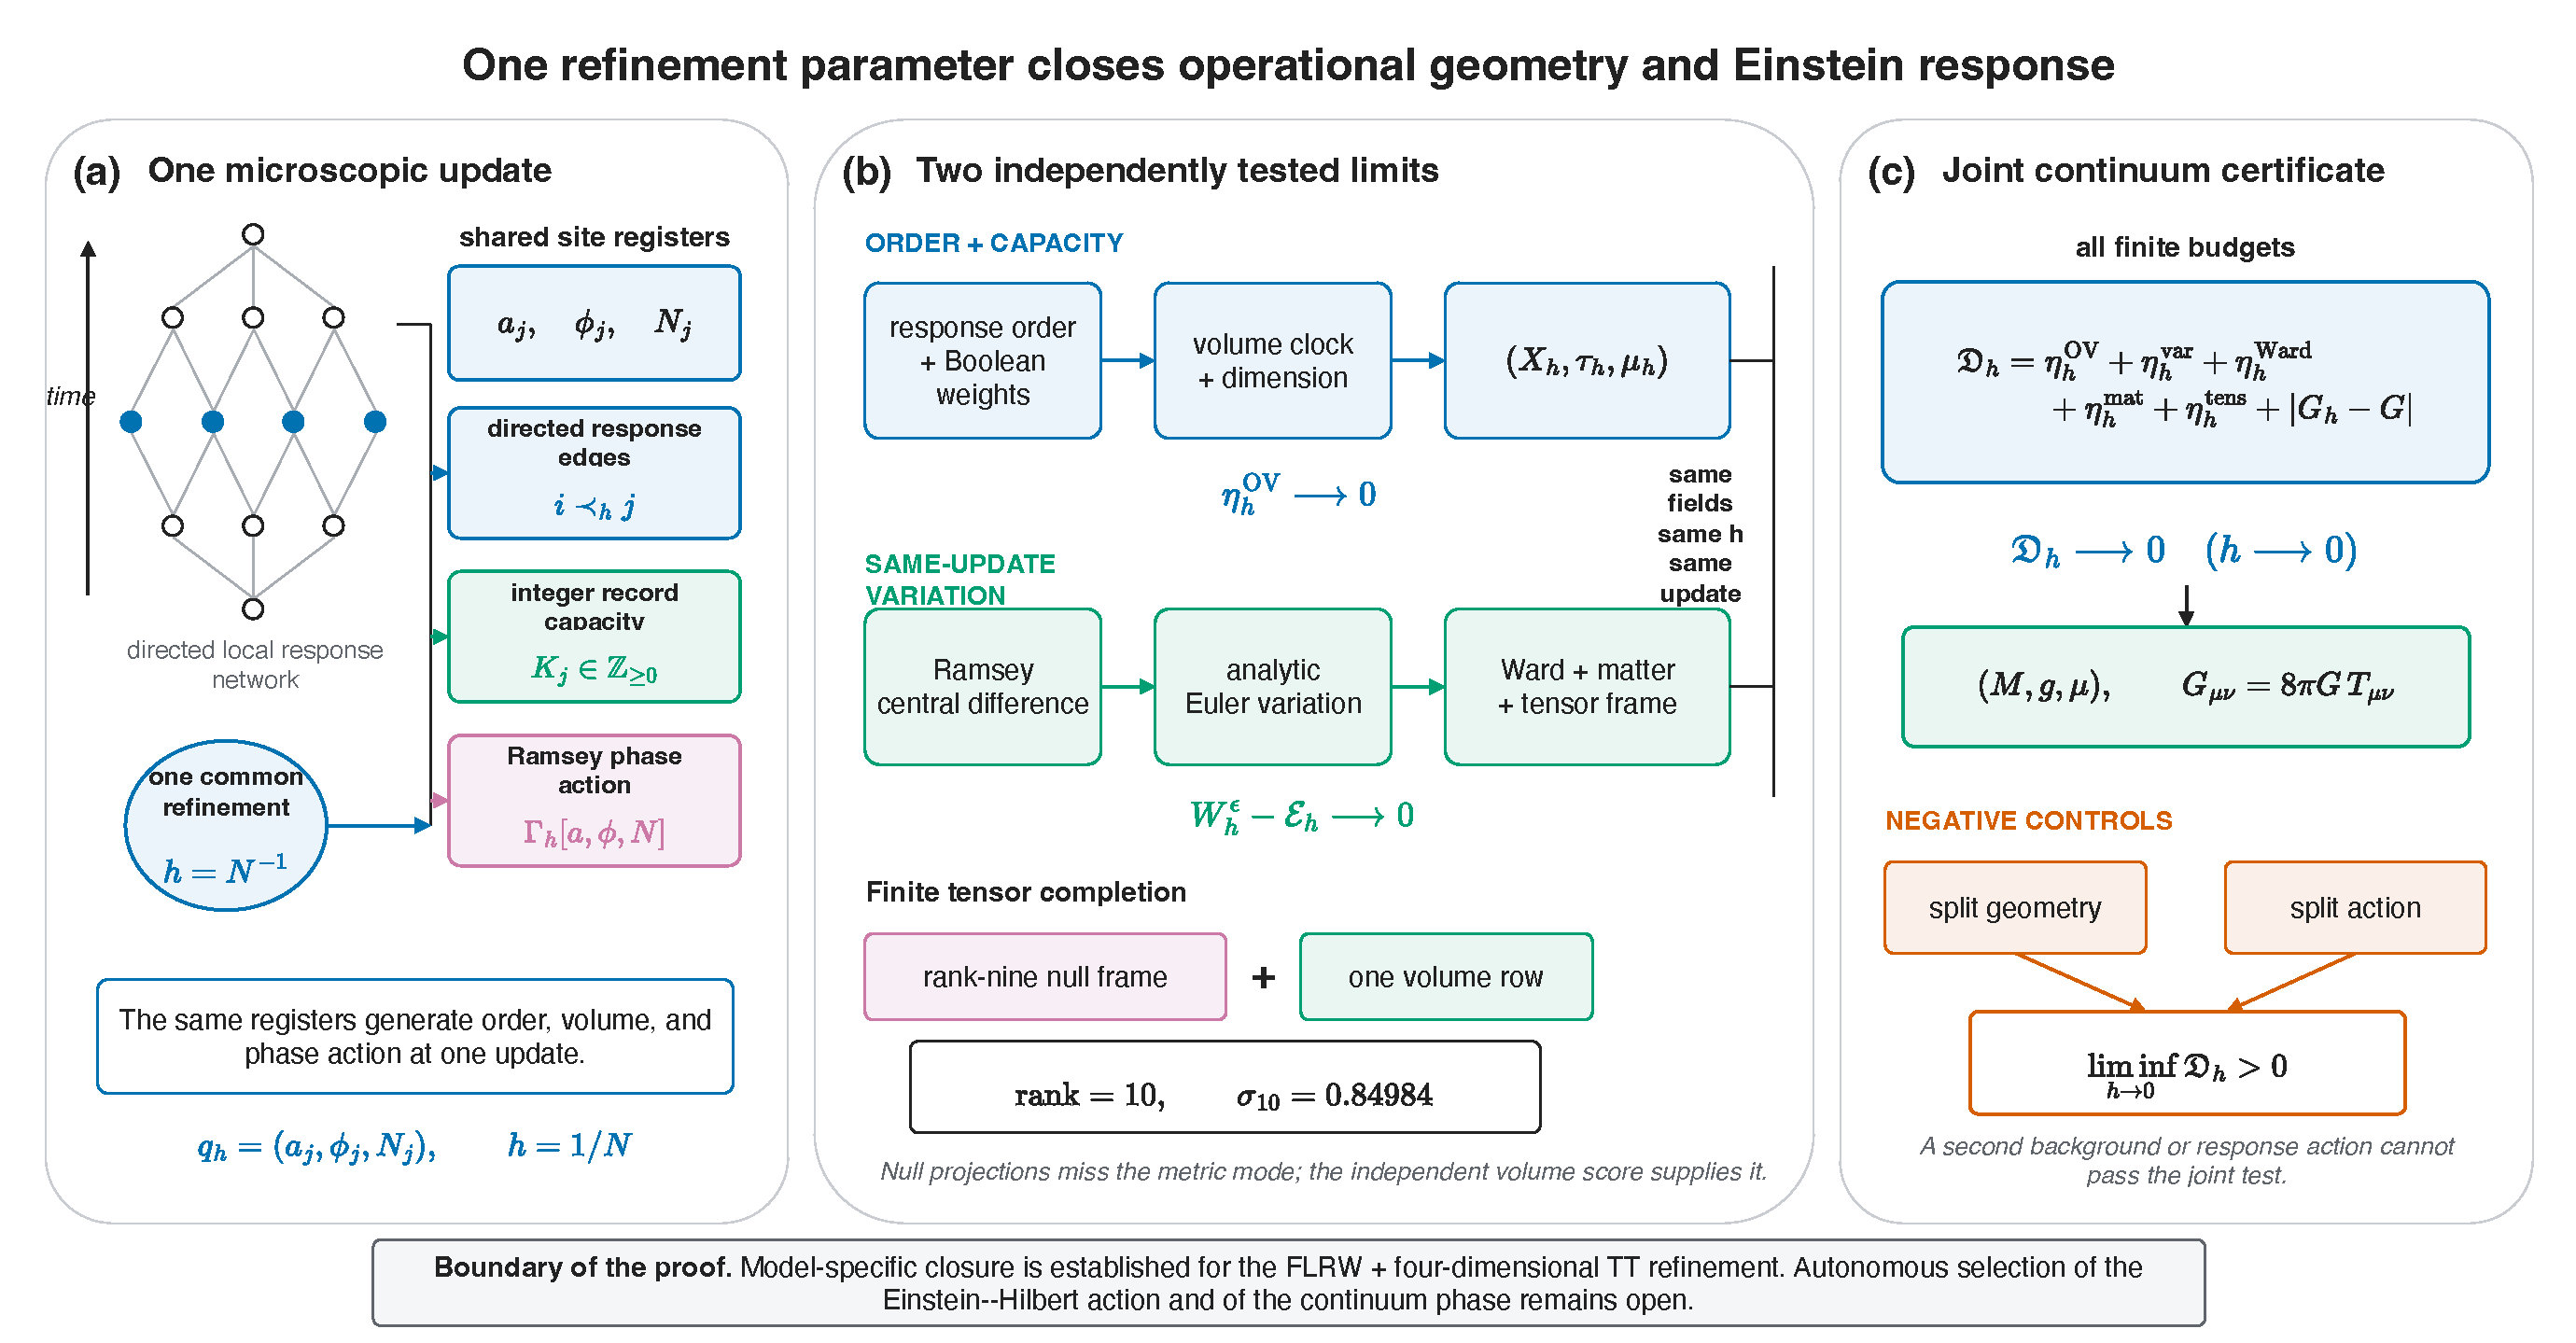
\includegraphics[width=0.97\linewidth]
 {figures/rqcp_qg_unified_continuum_v1.pdf}
 \caption{\textbf{Unified operational continuum limit.}
 Panel (a) records the common microscopic data: the same
 \(q_h=(a_j,\phi_j,N_j)\) and \(h=N^{-1}\) generate directed response
 records, integer Boolean capacities, and a Ramsey phase action.
 Panel (b) keeps geometry reconstruction and analytic variation independent;
 rank-nine null data plus one volume row determine all ten components of a
 symmetric four-tensor.  Panel (c) collects every finite defect before the
 limit is taken.  Split-geometry and split-action controls retain a nonzero
 floor.  The gray boundary box lists the inputs that the theorem does not
 select.  The figure is vector and its editable source is distributed with
 the companion manuscript.}
 \label{fig:unified-continuum-mechanism}
\end{figure}
\end{landscape}

\subsection{The joint finite certificate}

Let \(\eta_h^{\rm OV}\) bound the measured Lorentzian reconstruction error,
\(\eta_h^{\rm var}\) the error made by interchanging variation and
refinement, \(\eta_h^{\rm Ward}\) the finite Noether defect,
\(\eta_h^{\rm mat}\) the independently evaluated matter equation residual,
and \(\eta_h^{\rm tens}\) the error in completing the symmetric metric Euler
tensor from operational projections.  Let \(B_h\) be the compatible finite
divergence.  Taylor's formula applied to
Eq.~\eqref{eq:unified-ramsey-score} gives
\begin{equation}
 \|W_h^\varepsilon-{\cal E}_h\|_h
 \le\frac{\varepsilon^2}{6}M_{0,h},
 \qquad
 \|B_h(W_h^\varepsilon-{\cal E}_h)\|_h
 \le\varepsilon^2M_{1,h}.
 \label{eq:unified-central-difference}
\end{equation}
The second bound is imposed on the differentiated remainder field itself;
the cruder estimate \(\|B_h\|M_{0,h}\) can lose a power of \(h\).

At each event, contract a symmetric tensor with a finite set of normalized
null rows
\(A_\ell[X]=X_{\mu\nu}\ell^\mu\ell^\nu\).  These rows have rank at most nine
in four dimensions because they annihilate the metric direction.  Adding
one normalized volume row \(A_V[X]=g^{\mu\nu}X_{\mu\nu}\) gives a full frame
\(A_h\).  If
\(\sigma_{\min}(A_h)\ge\sigma_*>0\), then
\begin{equation}
 \|X\|_2\le\sigma_*^{-1}\|A_hX\|_2 .
 \label{eq:unified-frame-bound}
\end{equation}
The volume score is thus information-theoretically nonredundant; no further
null direction can replace it.

Define
\begin{align}
 {\mathfrak D}_h={}&
 \eta_h^{\rm OV}
 +\Delta_h^{\rm same}
 +\eta_h^{\rm var}
 +\frac{\varepsilon_h^2}{6}M_{0,h}
 +\varepsilon_h^2M_{1,h}\nonumber\\
 &+\eta_h^{\rm Ward}
 +\eta_h^{\rm mat}
 +\sigma_*^{-1}\eta_h^{\rm tens}
 +|G_h-G|.
 \label{eq:unified-certificate}
\end{align}
Every term is a finite-resolution quantity.  In particular, the Newton
coefficient is not hidden in the tensor norm: if it is supplied rather than
derived, the term \(|G_h-G|\) records that fact.

\begin{theorem}[Unified operational continuum limit]
\label{thm:unified-operational-continuum}
Let \(\{{\cal R}_h\}\) be a single-update refinement family on a compact
globally hyperbolic test region.  Suppose:
\begin{enumerate}[label=(U\arabic*)]
\item the order--volume reconstruction obeys
\(d_{\mathrm{mL}}[{\cal X}_h,({\cal M},\tau_g,\mu_g)]
\le\eta_h^{\rm OV}\to0\);
\item sampling and interpolation are stable and
\(\|{\cal I}_h{\cal E}_h-{\cal E}(g,\psi)\|_{H^{-1}}
\le\eta_h^{\rm var}\to0\);
\item Eq.~\eqref{eq:unified-central-difference} holds and
\(\varepsilon_h^2(M_{0,h}+M_{1,h})\to0\);
\item the null-plus-volume frame satisfies
\(\sigma_{\min}(A_h)\ge\sigma_*>0\); and
\item the Ward, matter, tensor, and coupling errors in
Eq.~\eqref{eq:unified-certificate} vanish.
\end{enumerate}
Then the operational geometry and response converge jointly:
\begin{align}
 d_{\mathrm{mL}}[{\cal X}_h,({\cal M},\tau_g,\mu_g)]
 &\le {\mathfrak D}_h,\label{eq:unified-geometry-limit}\\
 \|{\cal I}_hW_h^{\varepsilon_h}-{\cal E}(g,\psi)\|_{H^{-1}}
 &\le C_{\cal I}{\mathfrak D}_h .
 \label{eq:unified-dynamics-limit}
\end{align}
If a compactly convergent sequence also has vanishing operational score,
\(\|{\cal I}_hW_h^{\varepsilon_h}\|_{H^{-1}}\to0\), then
\({\cal E}(g,\psi)=0\) on the same metric--measure geometry selected by
Eq.~\eqref{eq:unified-geometry-limit}.  For the Einstein--matter action,
\begin{equation}
 G_{\mu\nu}[g]+\Lambda g_{\mu\nu}
 =8\pi G\,T_{\mu\nu}[g,\psi],
 \qquad {\cal E}_{\psi}(g,\psi)=0
 \label{eq:unified-einstein-limit}
\end{equation}
in the weak sense.
\end{theorem}

\begin{proof}
Insert \({\cal E}_h\) between the Ramsey score and the continuum Euler
covector.  Stable interpolation, the two estimates in
Eq.~\eqref{eq:unified-central-difference}, and variational consistency give
the projected response bound.  The rank-nine null frame reconstructs the
nonmetric tensor sector; Eq.~\eqref{eq:unified-frame-bound} and the volume
row add the missing metric component.  The Ward and matter terms control the
finite conservation and off-shell matter defects.  The order--volume term
fixes the continuum geometry, and
\(\Delta_h^{\rm same}\) prevents a second geometry from entering the phase
branch.  The triangle inequality yields
Eq.~\eqref{eq:unified-dynamics-limit}.  Passing to a compact limit of
vanishing operational scores gives
Eq.~\eqref{eq:unified-einstein-limit}.  No unproved interchange of
variation and limit occurs; its entire cost is \(\eta_h^{\rm var}\).
\end{proof}

\begin{corollary}[Split-limit rejection]
\label{cor:unified-split-rejection}
If \(\liminf_{h\to0}\Delta_h^{\rm same}>0\), or if the Ramsey branch uses
\(\Gamma_h+Q_h\) while the analytic branch varies \(\Gamma_h\) and
\(\liminf\|{\cal I}_hDQ_h\|>0\), then
\(\liminf_{h\to0}{\mathfrak D}_h>0\).
\end{corollary}

\subsection{Explicit FLRW--tensor realization}

The theorem is realized on
\begin{equation}
 {\cal M}=[1,2]\times\mathbb T^3,\qquad
 \mathrm ds^2=-\mathrm dt^2+a(t)^2\mathrm d\bm x^2 ,
 \label{eq:unified-flrw-metric}
\end{equation}
with \(8\pi G=1\) and
\begin{equation}
 a(t)=t^{1/3},\qquad
 \phi(t)=\sqrt{\frac23}\log t,\qquad
 N(t)=1 .
 \label{eq:unified-flrw-solution}
\end{equation}
For \(h=N^{-1}\), the same samples
\(q_h=(a_j,\phi_j,N_j)\) determine all three branches.  With
\(\eta(t)=\tfrac32t^{2/3}\), the response order is
\begin{equation}
 (j,\bm n)\prec_h(k,\bm m)
 \quad\Longleftrightarrow\quad
 j<k,\qquad
 h\,d_{\mathbb T^3}(\bm n,\bm m)
 <\eta(t_k)-\eta(t_j).
 \label{eq:unified-flrw-order}
\end{equation}
Each four-cell carries the Boolean capacity and weight
\begin{equation}
 C_j=\operatorname{round}\!\left[(N^3+1)a(t_{j+1/2})^3\right],
 \qquad
 w_j=h^4\frac{C_j}{N^3+1}.
 \label{eq:unified-capacity}
\end{equation}
The weighted counting measure converges to
\(a^3\,\mathrm dt\,\mathrm d^3x\).  Applying the intrinsic local
volume clock of Sec.~\ref{sec:generic-order-volume} on pieces of proper size
\(r_h\) gives
\begin{equation}
 |\widehat\tau_h-\tau_g|
 \le C\left(r_h^2+\frac{h}{r_h}+h^2+h^3\right).
 \label{eq:unified-order-volume-rate}
\end{equation}
The terms arise from small-diamond curvature, the lattice boundary shell,
midpoint quadrature, and capacity quantization.  Choosing
\(r_h=h^{1/3}\) gives the conservative complete clock rate
\(\eta_h^{\rm OV}=O(h^{2/3})\); the weak measure and local homogeneous metric
converge faster.

The phase branch uses the same samples in the midpoint
Einstein--massless-scalar functional
\begin{align}
 \Gamma_h[a,\phi,N]
 =\sum_{j=0}^{N-1}h\bigg[
 -\frac{3\bar a_j}{N_j}
  \left(\frac{a_{j+1}-a_j}{h}\right)^2
 +\frac{\bar a_j^3}{2N_j}
  \left(\frac{\phi_{j+1}-\phi_j}{h}\right)^2
 \bigg],
 \label{eq:unified-discrete-action}\\
 \bar a_j=\tfrac12(a_j+a_{j+1}).
 \nonumber
\end{align}
It generates the diagonal Ramsey phase and is varied independently to
obtain \({\cal E}_h\).  The variational, finite Ward, and scalar Euler
residuals converge at second order.  A periodic \(N^4\)
transverse-traceless sector supplies genuinely four-dimensional tensor
data.  Thirty rational null directions give rank nine; adding the volume
row gives rank ten with
\begin{equation}
 \sigma_{10}=0.8498365856 .
 \label{eq:unified-frame-sigma}
\end{equation}
The TT Ramsey--Euler defect is below \(3.01\times10^{-14}\), and the tensor
reconstruction error converges with fitted power \(1.951\).

\begin{figure}[htbp]
 \centering
 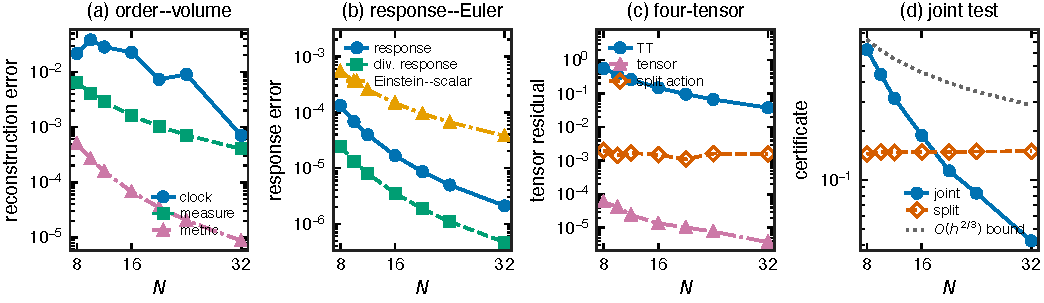
\includegraphics[width=\linewidth]
 {figures/rqcp_qg_unified_continuum_data_v1.pdf}
 \caption{\textbf{Deterministic synthetic refinement tests for the unified
 continuum certificate.}
 All panels use the common sizes \(N=8,10,12,16,20,24,32\).
 The order--volume observables, independent Ramsey/variation defects, and
 four-dimensional tensor residuals decrease under the same refinement.
 The complete certificate falls from \(0.630515\) to \(0.042254\), with
 fitted power \(1.949\) over the displayed sizes.  The gray
 \(O(h^{2/3})\) line is the conservative analytic envelope for the complete
 volume clock, not a fitted exponent.  Deliberately split geometry and
 action branches remain between \(0.1437\) and \(0.1498\).  These are
 reproducible synthetic calculations, not experimental data.}
 \label{fig:unified-continuum-data}
\end{figure}

The numerical archive contains 467 independent algebraic, refinement,
conditioning, split-control, and figure-data checks with no failed test.
The measured joint certificate decreases from \(0.630515\) at \(N=8\) to
\(0.042254\) at \(N=32\).  The split control remains between \(0.1437\) and
\(0.1498\), the minimum theorem-bound/actual-tensor-error ratio is \(1.7405\),
and the fitted powers of the Ward, Einstein--scalar, TT, tensor, and joint
errors are respectively \(1.898\), \(1.927\), \(1.945\), \(1.951\), and
\(1.949\).  These fitted powers diagnose this smooth family; the proved
order--volume statement remains the conservative
\(O(h^{2/3})\) estimate in
Eq.~\eqref{eq:unified-order-volume-rate}.

\subsection{Boundary of the result}

The model removes the possibility that the order--volume and
Einstein-response limits are mutually incompatible merely because they use
different discrete fields or different refinement maps.  It establishes a
nonempty, falsifiable realization in which one \(h\), one register family,
one capacity measure, and one phase action pass a common finite certificate.
It does \emph{not} remove the general assumptions \(A9V\) or \(A11\).
Specifically:
\begin{enumerate}
\item the four-dimensional manifold and \(\mathbb T^3\) topology are inputs;
\item the Einstein--Hilbert plus massless-scalar action is supplied, not
selected by a less structured microscopic channel;
\item the integer capacity unit and \(G_h=G\) are fixed microscopically;
\item the proof covers nonlinear homogeneous geometry and local
four-dimensional TT refinement, not arbitrary nonlinear inhomogeneous
spacetimes;
\item quantum fluctuations, renormalization, autonomous clock selection, and
a probability-law continuum limit remain open.
\end{enumerate}
The separate same-link construction in
Sec.~\ref{sec:same-link-induced-gravity} removes the supplied-curvature-action
input and controls large-\(N_s\) quantum fluctuations only for one
fixed-volume TT polarization at fixed microscopic spacing.  It does not
upgrade the present FLRW--Einstein--matter theorem to a general quantum
probability-law continuum limit.
The result is therefore a \emph{model-specific unified continuum closure}.
The general target remains one autonomous local quantum dynamics that
selects its manifoldlike phase, capacity-density law, gravitational action,
and regulator-independent Newton coefficient.


\section{Open bridge II: modular response and gravitational dynamics}
\label{sec:updated-gravity-bridge}

\textbf{Status: \StatusAbstract\ for the relative-entropy identity;
\StatusNumerical\ for the free-lattice certificate;
\StatusModel\ for the affine linearized closure, finite nonlinear
remainder theorem, and balanced quadratic regulator limit;
\StatusModel\ for the separate free positive-Hilbert spectral-balance
realization on supplied finite graph ensembles; \StatusOpen\ for a partial
interacting Ward identity, dynamically generated refinement measure,
nonlinear Einstein dynamics, Lorentzian RG protection, and a common
nonperturbative measure.}

Let \(\mathcal M_D\) be a local algebra and
\(\omega_D^0\) a faithful reference state.  In a Type-I regulator,
\(K_D^0=-\log\rho_D^0\), and
\begin{equation}
 S(\rho_s\|\rho_0)
 =\Delta\langle K_D^0\rangle_s-\Delta S_s .
 \label{eq:updated-relative-entropy}
\end{equation}
The first variation at \(s=0\) vanishes:
\begin{equation}
 \delta S=\delta\langle K_D^0\rangle .
 \label{eq:updated-first-law}
\end{equation}
For Type-III algebras the corresponding statement uses Araki relative
entropy and the relative modular operator \cite{Araki}.  Equation
\eqref{eq:updated-first-law} is an algebraic theorem.  It does not identify
\(K_D^0\) with stress-energy or curvature.

The lattice result in Sec.~\ref{sec:loop-modular} asks a narrower,
operationally well-posed question.  For a free critical interval, can the
linear modular response in a fixed physical frequency band be replaced by a
sparse local boost generator with a certified error?  The answer is yes in
that model.  The band is chosen from the local operator \(B_N\), its retained
dimension grows with the cutoff, and the response error is bounded in trace
norm.  The range-three correction has a frozen no-refit numerical validation.

To reach a gravitational equation, a common microscopic model must still
establish:
\begin{enumerate}[label=(E\arabic*)]
\item local diamond algebras on the response-generated geometry;
\item a modular-to-boost limit at fixed physical bandwidth in more than one
spatial dimension;
\item several independent null directions, so that an integrated scalar
projection does not masquerade as a tensor equation;
\item a transverse information density whose normalization determines
\(1/(4G_{\rm eff}\hbar)\), rather than importing \(G\);
\item a nonlinear focusing or area-response identity with controlled lattice,
localization, and state errors;
\item same-update decay of both constitutive defects in
\eqref{eq:finite-constitutive-certificate}, controlled finite symmetry and
matter-equation residuals, and the uniform conditioning required by
Theorem~\ref{thm:ward-bianchi-completion}.
\end{enumerate}
The affine null-wire regulator of
Sec.~\ref{sec:affine-null-wire-closure} realizes model versions of
(E1)--(E6): translated lattice subdiamonds, a fixed-band transverse wire
bundle, 30 null directions, boundary record entropy, a discrete focusing
recurrence, conserved wire stress, and an exact central-difference Bianchi
identity.  The qualifications are essential.  Its ``higher-dimensional''
matter is a direct sum of decoupled wires; the response cone and area
calibration are specified; and the equation is linearized around the
reconstructed constant metric.

The finite nonlinear bridge of
Sec.~\ref{sec:nonlinear-information-focusing} removes two further
approximations without claiming the remaining implication.  It replaces the
entropy first law by Eq.~\eqref{eq:nonlinear-finite-information}, the scalar
linear focusing law by the matrix identities
\eqref{eq:nonlinear-riccati}--\eqref{eq:nonlinear-area-update}, and the flat
rank certificate by Eq.~\eqref{eq:nonlinear-curved-rank}.  Its output is the
defect equation \eqref{eq:nonlinear-null-defect}.  The missing content of
(E6) is precisely the microscopic Ward relation
\eqref{eq:nonlinear-ward-target}, not an unspecified collection of
``higher-order corrections.''

The finite completion theorem of
Sec.~\ref{sec:ward-bianchi-completion} sharpens (E6) further.  Once the tensor
defined by the null defect is the geometric Euler covector, its nonmetric
part, divergence, local scalar mode, measurement noise, symmetry defect, and
off-shell matter residual enter the explicit bound
\eqref{eq:ward-bianchi-completion}.  The theorem therefore removes a
qualitative tensor-completion assumption but not the constitutive
identification or its uniform dynamical suppression.

The same-update theorem of Sec.~\ref{sec:same-update-einstein} closes that
identification for one declared local phase action and fixes the remaining
constant metric mode with a volume score.  Thus (E6) is complete in the FLRW
and \(L^4\) transverse-traceless regulators at finite resolution.  What
remains open in the generic program is not another tensor inversion: it is
the dynamical selection of this Einstein--matter phase from the preceding
record--geometry update, together with interacting modular input and uniform
regulator control.

Only after (E1)--(E6) are available would the familiar conditional chain
\begin{equation}
 \delta S_{\rm alg}
 =\delta\langle K\rangle
 \longrightarrow
 \delta A+4G_{\rm eff}\hbar\,\delta S_{\rm bulk}=0
 \longrightarrow
 \delta G_{\mu\nu}=8\pi G_{\rm eff}\delta T_{\mu\nu}
 \label{eq:updated-einstein-chain}
\end{equation}
become an internal derivation.  It is internal to the affine regulator under
the hypotheses of Theorem~\ref{thm:affine-model-closure}; it remains
conditional in the generic program.  The last two arrows are closely related
to thermodynamic and entanglement-equilibrium routes to the Einstein equation
\cite{Jacobson1995,Jacobson2015}; citing those routes alone would not supply
the microscopic area density, separating null probes, or focusing identity
constructed in the regulator.

At finite exchange and curvature, the corresponding nonlinear chain is not
obtained by replacing every \(\delta\) in
Eq.~\eqref{eq:updated-einstein-chain} with \(\Delta\).  The positive
\(\mathcal R_{\rm info}\), nonlinear optical remainder, modular defect, and
localization error must instead satisfy
Eqs.~\eqref{eq:nonlinear-null-defect} and
\eqref{eq:nonlinear-ward-target}.  This distinction is the main advance of
the second bridge and the reason the full nonlinear claim remains open.

\section{de Sitter response: benchmark, inverse theorem, and non-emergence}
\label{sec:updated-desitter}

\textbf{Status: \StatusNumerical/\StatusConditional.}
Two de Sitter constructions appeared in the earlier manuscript and should
not be conflated.

First, a Poisson sprinkling of a de Sitter causal diamond, equipped with
response gates and record dephasing, is a consistency benchmark.  If the
continuum geometry is used to generate the graph, recovering de Sitter
relations shows that the model class is nonempty and that the discretization
can preserve the intended symmetries.  It does not show that the geometry
emerges.

Second, the quantum-field inverse theorem of
Sec.~\ref{sec:loop-lorentz} treats the radius as unknown.  The data are Ramsey
coherences, not coordinate distances, and the rank-five condition fixes
\[
 R^2=(\mathbf1^TA^{-1}\mathbf1)^{-1}.
\]
This is a genuine output within a specified background and state family.
Its strongest tests are redundant sextuple radii, Lorentzian inertia,
target hyperboloid norms, and target pairs withheld until the estimator is
frozen.  Failure of any of those tests rejects the assumed kernel--geometry
pair.  This result builds on the established use of field propagators and
localized quantum measurements as geometric probes
\cite{SaravaniAslanbeigiKempf2016,PercheMartinMartinez2022}; it is not a
claim to have invented response-based geometry.

The two constructions can support a future closed loop only if a single
background-free process produces both the laboratories and the field
response used by the inverse theorem.  Until then, the correct claim is
\[
 \text{physical quantum response can infer an unknown de Sitter scale},
\]
not
\[
 \text{de Sitter spacetime has been derived from the RQCP dynamics}.
\]

\section{Central charge, metric volume, and vacuum counterterms}
\label{sec:updated-vacuum}

\textbf{Status: \StatusModel\ for the charge center;
\StatusConditional\ for fixed-volume cancellation;
\StatusOpen\ for cosmology.}

The local model of Sec.~\ref{sec:loop-center} proves
\begin{equation}
 \ker\mathcal L^*
 =\operatorname{span}\{P_0,\ldots,P_N\},
 \qquad
 \Delta\ge\min\{\gamma/2,\eta\lambda_2(L_G)\}.
 \label{eq:updated-charge-center}
\end{equation}
This is the part that is derived.  The projectors \(P_v\) are the complete
fixed observable algebra of a local Lindbladian, and weak homogeneous flips
lift the degeneracy into an exact Ehrenfest spectrum.  No global center
variable is appended to obtain this result.

\subsection{The conditional fixed-volume identity}

Suppose, in addition, that \(v\) converges to Euclidean four-volume and that
one computes normalized response in a fixed sector:
\[
 \mathcal W_v[J]=\log Z_v[J]-\log Z_v[0].
\]
If a matter loop adds a source-independent term \(c_0m^4v\), then
\begin{equation}
 Z_v[J]\mapsto e^{-c_0m^4v}Z_v[J]
 \quad\Longrightarrow\quad
 \mathcal W_v[J]\mapsto\mathcal W_v[J].
 \label{eq:updated-a0-cancel}
\end{equation}
Every connected \(J\)-derivative is unchanged.  This is more informative
than cancellation of a global state-vector phase, because it concerns a
normalized generating functional.

The selectivity is equally important.  For a regulated local matter theory,
\begin{equation}
 \Gamma_{\rm eff}[g]
 =\int\!\sqrt g\,
 \left(c_0m^4+c_1m^2R+c_2R^2
 +c_3R_{\mu\nu}R^{\mu\nu}+\cdots\right).
 \label{eq:updated-heat-kernel}
\end{equation}
Only the \(c_0m^4v\) term is constant on a fixed metric-volume sector.
Curvature, anomaly, boundary, and field-dependent terms remain in connected
response and undergo ordinary effective-field-theory renormalization.

\subsection{The missing central-volume bridge}

Equation~\eqref{eq:updated-a0-cancel} becomes relevant to gravity only after
proving all of the following in one model:
\begin{enumerate}[label=(V\arabic*)]
\item an additive microscopic charge with the exact center property
\eqref{eq:updated-charge-center};
\item convergence of that charge to metric four-volume, including units and
finite-size error;
\item sectorwise normalization derived from process composition rather than
imposed as a choice of ensemble;
\item a gravitational response map that is local within a sector and cannot
measure cross-sector weights;
\item preservation of (V1)--(V4) under coarse graining and matter
counterterms.
\end{enumerate}
The present work establishes (V1) for a hard-core channel and the algebraic
consequence of (V2)--(V3) if they hold.  It does not establish (V2)--(V5).

The earlier action with a hand-introduced variable \(\lambda_R\) is therefore
best read as a comparison with sequestering or unimodular constructions, not
as a microscopic result.  Likewise,
\(\rho_\Lambda\propto M_{\rm Pl}^2L_R^{-2}\) is dimensional scaling unless
the central stiffness, the response length \(L_R\), and their coupling to
curvature are all derived.  The present construction makes no prediction for
\(\Lambda\) \cite{FiolGarriga2010,KaloperPadilla,WeinbergCC}.

\section{Matter reconstruction as a sequence of open classification
problems}
\label{sec:updated-matter}

\textbf{Status: \StatusOpen.}
The earlier long form attached gauge registers to causal links and imposed a
finite spectral triple.  Both are useful target constructions, but neither
derives the Standard Model from the foundational channel.

\subsection{Gauge symmetry from influence sectors}

The nontrivial target is to begin with localized endomorphisms or residual
influence sectors \(\{\rho_a\}\) and prove that they form a rigid symmetric
tensor \(C^*\)-category,
\begin{equation}
 \rho_a\otimes\rho_b
 \simeq\bigoplus_cN_{ab}^{\ \ c}\rho_c ,
 \label{eq:updated-fusion}
\end{equation}
with conjugates, intertwiners, locality, and a faithful fiber functor.
Tannaka--Krein or Doplicher--Roberts reconstruction would then identify a
compact group \(G\) with
\(\mathcal C_{\rm infl}\simeq\operatorname{Rep}(G)\)
\cite{DoplicherRoberts}.  The theorem to be
proved is the emergence of the category from one local channel, not the
known reconstruction result once the category is supplied.

The first credible milestone is one finite non-Abelian group or \(SU(2)\) in
an explicit model, together with an operational holonomy or charge-fusion
observable.  Attaching \(U_{xy}\) by hand and obtaining
\(U_p\simeq\exp(iF_{\mu\nu}\Sigma^{\mu\nu})\) shows how a given gauge register
has a continuum limit; it does not explain why the register or group exists.

\subsection{Chiral matter on causal defects}

A domain-wall Dirac operator can carry an index, and that index can protect
chiral zero modes.  The required RQCP result is a discrete causal or
non-Hermitian Dirac operator whose spectral flow, anomaly inflow, and index
remain stable under the same coarse graining that produces the causal
records.  Selecting topological data with \(\operatorname{Index}=3\) does
not explain three generations.  The first closed result should instead prove
index stability under disorder, weak nonunitarity, and record RG; a later
dynamical selection problem may ask why a particular index is preferred.

\subsection{Finite noncommutative geometry}

The algebra
\[
 \mathcal A_F=\mathbb C\oplus\mathbb H\oplus M_3(\mathbb C)
\]
is highly constrained once the axioms of a finite real spectral triple,
unimodularity, anomaly cancellation, and a representation are imposed.  In
RQCP-QG these are selection conditions on a candidate residual algebra.
They are not presently consequences of the influence-channel flow.  The
correct dependency is
\[
 \text{derived residual sector category}
 \longrightarrow
 \text{classification constraints}
 \longrightarrow
 \text{candidate matter algebra},
\]
with the first arrow still open.

\section{Response horizon and dark condensate: phenomenological branches}
\label{sec:updated-cosmology}

\textbf{Status: \StatusOpen.}
The response-horizon and response-superfluid constructions are retained as
testable long-horizon branches, not as support for the foundational chain.

\subsection{Response-horizon attractor}

For
\begin{equation}
 F_R(L)=\alpha M_{\rm Pl}^2H^2L^3
 -\beta M_{\rm Pl}^2HL^2+\cdots ,
 \label{eq:updated-horizon-free-energy}
\end{equation}
stationarity gives
\[
 L_R=\frac{2\beta}{3\alpha}H^{-1}.
\]
Imposing first-law matching at \(L=H^{-1}\) and then deriving
\(L_R=H^{-1}\) is circular.  A microscopic result must compute
\(\alpha\) and \(\beta\) independently of the desired radius, show
\(F_R''(L_R)>0\), derive the relaxation rate, and include matter and anomaly
corrections.  Until that calculation is performed,
\(3\alpha=2\beta\) is a model check, not a prediction.

\subsection{Response condensate}

The hydrodynamic ansatz
\[
 S_R=\int\!P_R(X)-\alpha_b\int\!\varphi\rho_b+\cdots
\]
can reproduce baryonic scaling if
\(P_R(X)\propto X\sqrt{|X|}\), as in the superfluid-dark-matter mechanism
\cite{BerezhianiKhoury}.  That exponent is currently an assumption.
A closed theory must derive the infrared singularity from a transfer spectrum
or response-charge critical point and produce at least one joint prediction
that cannot be adjusted independently, for example
\[
 \text{BTFR normalization}
 \longleftrightarrow
 \eta_{\rm slip}(k,z)
 \longleftrightarrow
 \text{cluster melting scale}.
\]
Rotation curves alone do not identify the mechanism.  Weak lensing,
clusters, the CMB, and linear growth must be treated by one parameter set,
with the condensate/normal-fluid boundary included.

\section{A status-preserving conditional synthesis}
\label{sec:updated-synthesis}

The value of a synthesis theorem is bookkeeping: it identifies a sufficient
set of bridges and prevents an omitted input from reappearing in the
conclusion.  It is not evidence that the bridges hold.

\begin{theorem}[Conditional composition with visible external inputs]
\label{thm:updated-conditional-synthesis}
Suppose:
\begin{enumerate}[label=(C\arabic*)]
\item the process-functional and influence-algebra hypotheses of
Sec.~\ref{sec:process-algebra} hold;
\item a local microscopic dilation has a controlled kinetic limit and an
infrared Boolean center;
\item a single model produces a locally finite causal order and a positive
information-volume measure with a Lorentzian metric--measure limit;
\item its local diamond algebras satisfy a modular-to-boost limit in a fixed
physical band, with a curved rank-nine family of local null probes;
\item the transverse information density fixes \(G_{\rm eff}\); the finite
information, modular, focusing, and localization remainders define the
geometric Euler covector of the same process; its symmetry and matter
residuals vanish uniformly; and the hypotheses of
Theorem~\ref{thm:ward-bianchi-completion} hold in a shrinking-diamond limit;
\item an additive central charge converges to metric four-volume and
sectorwise process normalization is stable under matter loops.
\end{enumerate}
Then the exact record events form a Boolean algebra; the continuum order and
measure determine the stated Lorentzian geometry; the relative-entropy first
law gives the tangent response, while the exact finite balance and
assumptions (C4)--(C5) imply the corresponding nonlinear Einstein dynamics;
and pure-volume counterterms cancel from normalized
fixed-sector response under (C6).
\end{theorem}

\begin{proof}
The Boolean conclusion follows from the center-projection theorem and the
assumed infrared convergence.  Assumption (C3) supplies, rather than derives,
the hypotheses of the relevant order--measure reconstruction theorem.
Equation~\eqref{eq:updated-first-law} gives the linear tangent statement.
At finite exchange, Theorem~\ref{thm:finite-nonlinear-remainder}, the
modular-to-boost limit, the constitutive Ward identification, and
Theorem~\ref{thm:ward-bianchi-completion} give the nonlinear gravitational
response under (C4)--(C5).  Finally, a pure volume counterterm
is constant in a fixed sector, so its multiplicative factor cancels between
\(Z_v[J]\) and \(Z_v[0]\).
No step proves (C3)--(C6); the theorem only records their consequences.
\end{proof}

\begin{remark}[Use of Theorem~\ref{thm:updated-conditional-synthesis}]
Theorem~\ref{thm:updated-conditional-synthesis} may be used to check that a
future microscopic model closes the whole chain.  It must not be cited as
evidence that RQCP-QG already derives a generic or nonlinear Einstein
equation, a cosmological constant, or a matter spectrum.
\end{remark}

The affine null-wire regulator supplies a model-specific linearized instance
of portions of (C3)--(C5).  The nonlinear finite-regulator theorem supplies
the exact information and optical identities and the curved null-frame
certificate.  Theorem~\ref{thm:capacity-reference-selection} additionally
selects the capacity-balanced reference for factorized tokens, but not from
the same nonlinear update and not for arbitrary correlated record geometry.
Theorem~\ref{thm:ward-bianchi-completion} additionally supplies the finite
tensor estimate and propagates nonzero response--Euler field and divergence
defects.  Theorem~\ref{thm:same-update-einstein} derives those two
constitutive budgets for one declared phase update, and
Theorem~\ref{thm:unified-operational-continuum} places that update and the
order--volume geometry on one common FLRW--TT refinement.  These model
theorems still do not select the Einstein--matter action, dimension,
capacity-density law, interacting modular dynamics, or universal \(G\).
They also do not supply (C6) or turn the generic continuum hypotheses into
background-independent theorems.  Accordingly, the warning in the preceding
remark continues to apply to autonomous quantum gravity, the cosmological
constant, and the matter spectrum.

\begin{landscape}
\section{Outstanding assumptions and decisive tests}
\label{sec:updated-ledger}

The remaining assumptions are ordered by logical dependence.  The last
column identifies an outcome that would falsify the proposed mechanism,
rather than merely leave its proof incomplete.

\small
\begin{longtable}{@{}P{0.17\linewidth}P{0.25\linewidth}
P{0.34\linewidth}P{0.16\linewidth}@{}}
\caption{Outstanding assumptions, the results needed to remove them, and
decisive failure tests.}
\label{tab:updated-assumption-ledger}\\
\toprule
Assumption & Required new result & Decisive observable or test & Failure
criterion\\
\midrule
\endfirsthead
\toprule
Assumption & Required new result & Decisive observable or test & Failure
criterion\\
\midrule
\endhead
One-pass memoryless bath
& Repeated-interaction limit with quantified initial correlations or finite
  bath reset
& Response-kernel error and information-backflow witness
& Recurrence survives on the claimed kinetic time\\
\addlinespace
Restricted block-cactus adjacency
& Bounded local cycle certificate or controlled nonlocal defect theory on a
  broader graph family
& Window DAG probability and critical order gap
& Long chordless cycles evade the certificate\\
\addlinespace
Autonomous adjacency and capacity-density law
& One closed dynamics selects the interaction support, enters a robust
  acyclic response phase, and derives the stable conversion from Boolean
  record capacity to the measure consumed by
  Theorem~\ref{thm:generic-order-volume-compactness}
& Adjacency susceptibility, cycle margin, capacity-density flow, and blind
  passage through the dimension, clock, covering, and topology certificates
& The operational gates fail persistently, or inequivalent capacity
  normalizations survive the same infrared dynamics\\
\addlinespace
Specified field state and de Sitter class
& Joint state--geometry identifiability or independent state calibration
& Redundant radii, inertia, hyperboloid norms, blind pairs
& State deformation passes every geometric test\\
\addlinespace
Free or decoupled-wire modular regulator
& Fixed-band bound in an interacting higher-dimensional model
& Multi-direction modular response and transverse density
& Error remains finite at fixed physical band\\
\addlinespace
Capacity-balanced boundary reference
& Extend Theorem~\ref{thm:capacity-reference-selection} from factorized tokens
  to correlated record geometry and couple it to the nonlinear update
& Correlated sector weights, modular area coefficient, contraction rate, and
  same-update Ward residual
& Selection fails without a record-number-dependent reset, or contraction
  vanishes under refinement\\
\addlinespace
Record count equals boundary area
& Derive \(\widehat A=a_0^2\widehat N\) from order--volume geometry and prove
  a universal refinement flow of \(a_0^2/\log q\)
& Blind area reconstruction and regulator flow of \(G_{\rm eff}\)
& Different microscopic tokenizations give inequivalent infrared
  coefficients\\
\addlinespace
Dynamical phase, action, and continuum selection
& Extend Theorems~\ref{thm:same-update-einstein} and
  \ref{thm:unified-operational-continuum} so that one
  record--matter--holonomy dynamics derives its effective phase action,
  rather than receiving the Einstein--matter form, selects its dimension and
  capacity law, and makes the finite symmetry and matter-equation residuals
  vanish uniformly in an interacting quantum refinement
& Direction-resolved information, modular, optical, constitutive, symmetry,
  matter, holonomy, order--volume, and coupling residuals, inserted into
  Eq.~\eqref{eq:unified-certificate}
& The infrared phase is not Einstein--Hilbert, the independent response and
  variation pipelines disagree, split controls pass, or the joint
  certificate stays finite under refinement\\
\addlinespace
Pre-caustic and integrated-diamond restriction
& Maslov-complete optical propagation and a uniform shrinking-diamond
  localization theorem
& Conjugate-point index, patch independence, and localization defect
& Area or tensor reconstruction becomes chart dependent at a caustic\\
\addlinespace
Regulator-dependent Newton normalization
& Renormalization or universality theorem for the boundary information
  coefficient
& The same infrared coefficient survives changes of record dimension and
  regulator
& Independent continuum extrapolations disagree\\
\addlinespace
Charge equals metric volume
& Scaling theorem from additive charge to four-volume
& Sector volume calibration and finite-size residual
& Charge fluctuations fail geometric extensivity\\
\addlinespace
Sectorwise vacuum normalization
& Derive the fixed-sector functional from process composition and perform a
  regulated matter-loop test
& \(a_0\) cancels while \(a_1,a_2,\ldots\) remain
& Source-dependent or curvature terms are spuriously removed\\
\addlinespace
Gauge category
& Residual influence sectors form a rigid symmetric tensor category
& Fusion, conjugates, intertwiners, and holonomy
& No stable category survives RG\\
\addlinespace
Chiral index and three generations
& RG-stable causal-defect Dirac index, followed by a separate selection
  mechanism
& Spectral flow and anomaly inflow under disorder
& Zero modes gap or index changes under allowed RG\\
\addlinespace
Horizon coefficient matching
& Compute \(\alpha,\beta,F_R''\), and relaxation from one model
& \(L_R/H^{-1}\) and attraction rate
& Equality requires imposing the target radius\\
\addlinespace
Dark equation of state
& Derive \(P_R(X)\) and a cross-scale parameter relation
& Rotation, lensing, clusters, CMB, and growth
& No common parameter region exists\\
\bottomrule
\end{longtable}
\end{landscape}

The order of work follows the dependency graph rather than the apparent
phenomenological reach:
\begin{enumerate}
\item submit and experimentally anchor the Boolean and memory loops;
\item unite Boolean records with dissipative causal order in one local
process;
\item extend the finite relational clock/order/volume model beyond its
compiled four-dimensional port language, then test the intrinsic inverse
geometry gates blindly;
\item extend and couple the factorized capacity-reference selection theorem,
derive the record--area map, and establish an interacting fixed-physical-band
modular response on that geometry;
\item couple record exchange, nonlinear Jacobi optics, Lorentz holonomy, and
matter transport so that the response tensor is the geometric Euler covector
of the same update and its finite symmetry and matter residuals vanish;
\item extend the common-refinement theorem from FLRW plus TT perturbations to
general nonlinear inhomogeneous four-dimensional configurations, quantum
fluctuations, and renormalized observables;
\item prove a caustic-complete, shrinking-diamond, regulator-independent
interacting limit and derive rather than impose the physical spectral
balance and Newton coefficient;
\item derive a metric-volume center and perform the selective loop
cancellation;
\item address gauge, chirality, horizon dynamics, and dark phenomenology
after their upstream inputs exist.
\end{enumerate}

\section{Conclusion}
\label{sec:updated-conclusion}

RQCP begins with an operational statement: response differences generate an
influence algebra, and its central projections are the jointly readable exact
events.  The explicit models studied here show that this statement has
nontrivial dynamics behind it.  Fresh-cell collisions produce the
dephasing--exchange kinetics microscopically; the resulting Lindbladian has
an exact Boolean charge algebra, a complete graph-dependent gap, and a
controlled metastable Markov reduction.  An absorbing noise field drives a
transition between quantum memory and Boolean records, and a
reversal-covariant defect dynamics produces a partial order before any
Lyapunov rank is introduced.

The order--volume result identifies the next mathematical step.  A certified
partial order and a positive additive record measure define an intrinsic
finite volume clock and, under compactness and identifiability conditions, a
Lorentzian metric--measure subsequential limit.  Smooth admissible limits
recover proper time, dimension, measure, and local topology with explicit
error and rejection criteria.  The theorem does not generate its order or
its absolute record-density unit.  The de Sitter Ramsey construction is
complementary: it determines an unknown curvature scale and blind invariants
from a physical field response, but only within a specified state and
geometry class.

The gravitational constructions establish several finite compatibility
results.  They control a physical modular band, null-frame inversion,
finite information balance, nonlinear optical propagation, Ward completion,
and the comparison between a measured response and the variation of the same
phase functional.  A common-refinement model places order, record measure,
and Einstein--matter response on one family of registers.  A same-link
determinant model derives a positive transverse-traceless two-derivative
kernel without a bare curvature term; relational histories, quadratic
constraint completion, and spectral balance extend this to a
regulator-independent Gaussian response.  These results demonstrate that
the required ingredients are mutually compatible in restricted models.
They do not select the dimension, microscopic program, nonlinear action,
interacting matter content, or continuum normalization.

The remaining foundational problem can be stated without reference to the
auxiliary regulators:
\begin{equation}
 \boxed{\begin{gathered}
 \text{one autonomous background-free process}
 \dashrightarrow
 \text{certified order + capacity-density law}\\
 \xrightarrow{\ \text{intrinsic volume clock}\ }
 (X,\tau,\mu)\\
 \dashrightarrow
 \text{selected Einstein phase + interacting quantum limit}.
 \end{gathered}}
 \label{eq:updated-open-core}
\end{equation}
The middle implication is proved under operational compactness and
identifiability conditions.  The first remains open because no general local
dynamics in the manuscript selects both adjacency and the absolute
capacity-density conversion.  The last is realized only in prescribed
finite or quadratic model families.  An autonomous completion must also
derive the gauge and clock structure, control nonlinear constraints and
renormalized observables, and show that the relevant limits are independent
of the microscopic regulator.

Projective causal histories and operator-growth rigidity constrain possible
solutions of the first implication, but they do not yet yield a covariant
non-Abelian geometry dynamics with backreaction.  Likewise, fixed-sector
normalization identifies a selective pure-volume cancellation, but a
metric-volume center and a regulated matter-loop calculation remain absent.
Gauge reconstruction, chirality, horizon dynamics, and dark phenomenology
therefore remain downstream questions.

The value of the framework at its present stage is the separation of these
claims.  Exact models establish the information and finite-response
mechanisms; conditional theorems specify how geometry and gravity would
follow under additional hypotheses; and the unresolved hypotheses are
accompanied by failure tests.  The framework will approach a microscopic
theory of quantum gravity only when the two dashed implications in
Eq.~\eqref{eq:updated-open-core} are obtained from the same dynamics.
